%% Template para dissertacao/tese na classe UFBAthesis
%% versao 1.0
%% (c) 2005 Paulo G. S. Fonseca
%% (c) 2012 Antonio Terceiro
%% (c) 2014 Christina von Flach
%% www.dcc.ufba.br/~flach/ufbathesis

%% Carrega a classe ufbathesis
%% Opcoes: * Idiomas
%%           pt   - portugues (padrao)
%%           en   - ingles
%%         * Tipo do Texto
%%           bsc  - para monografias de graduacao
%%           msc  - para dissertacoes de mestrado (padrao)
%%           qual - exame de qualificacao de mestrado
%%           prop - exame de qualificacao de doutorado
%%           phd  - para teses de doutorado
%%         * Media
%%           scr  - para versao eletronica (PDF) / consulte o guia do usuario
%%         * Estilo
%%           classic - estilo original a la TAOCP (deprecated) - apesar de deprecated, manter esse.
%%           std     - novo estilo a la CUP (padrao)
%%         * Paginacao
%%           oneside - para impressao em face unica
%%           twoside - para impressao em frente e verso (padrao)

% Atenção: Manter 'classic' na declaracao abaixo:
\documentclass[qual, classic, a4paper]{ufbathesis}

%% Preambulo:
\usepackage[utf8]{inputenc}

%\usepackage[authoryear]{natbib}
\usepackage{graphicx}
\usepackage{lipsum}
\usepackage{hyphenat}
\usepackage[usenames, dvipsnames, table]{xcolor}
\usepackage{booktabs}
\usepackage{pifont}
\usepackage{multirow}
\usepackage{listings} 
\usepackage{colortbl}
\usepackage{xfrac}
\usepackage[FIGTOPCAP]{subfigure}
\usepackage{tabularx}
\usepackage{ragged2e}
\usepackage{acronym}
\usepackage{float}
\usepackage{todonotes}
\usepackage{amssymb}
\usepackage{placeins}
\usepackage{arydshln}

\presetkeys%
    {todonotes}%
    {inline,backgroundcolor=yellow}{}
    
\usepackage{blindtext}

\usepackage{tikz}
\usetikzlibrary{arrows,shapes,positioning,shadows,trees}

% Siglas
\acrodef{AM}[AM]{{Aprendizado de Máquina}}
\acrodef{DE}[DE] {{Distância Euclidiana}}
\acrodef{FCD}[FCD] {{\textit {Fluxo de Dados Contínuos}}}
\acrodef{DN}[DN] {{\textit {Detecção de Novidade}}}

% Universidade
\university{Universidade Federal da Bahia}

% Endereco (cidade)
\address{Salvador}

% Instituto ou Centro Academico
\institute{Instituto de Matem\'{a}tica}

% Nome da biblioteca - usado na ficha catalografica
\library{Biblioteca Reitor Mac\^{e}do Costa}

% Programa de pos-graduacao
\program{Programa de P\'{o}s-Gradua\c{c}\~{a}o em Ci\^{e}ncia da Computa\c{c}\~{a}o}

% Area de titulacao
\majorfield{Ci\^{e}ncia da Computa\c{c}\~{a}o}

% Titulo da dissertacao
\title{Aplicando redes de função de base radial para detecção de mudanças de conceito em fluxos contínuos de dados}

% Data da defesa
% e.g. \date{19 de fevereiro de 2013}
\date{03 de Abril de 2019}
% e.g. \defenseyear{2013}
\defenseyear{2019}

% Autor
% e.g. \author{Jose da Silva}
\author{Ruivaldo Azevedo Lobão Neto}

% Orientador(a)
% Opcao: [f] - para orientador do sexo feminino
% e.g. \adviser[f]{Profa. Dra. Maria Santos}
\adviser{Ricardo Ara\'{u}jo Rios}

% Orientador(a)
% Opcao: [f] - para orientador do sexo feminino
% e.g. \coadviser{Prof. Dr. Pedro Pedreira}
% Comente se nao ha co-orientador
%\coadviser{Nome Completo do CO-ORIENTADOR}

%% Inicio do documento
\begin{document}

\pgcompfrontpage

%% Parte pre-textual
\frontmatter

\pgcomppresentationpage

%%%%%%%%%%%%%%%%%%%%%%%%%
% Ficha catalografica
%%%%%%%%%%%%%%%%%%%%%%%%%

%\authorcitationname{Silva, Mirlei Moura da } % e.g. Terceiro, Antonio Soares de Azevedo
%\advisercitationname{Sobrenome, Nome do ORIENTADOR} % e.g. Chavez, Christina von Flach Garcia
%\coadvisercitationname{Sobrenome, Nome do CO-ORIENTADOR} % e.g. Mendonca, Manoel Gomes de
%\catalogtype{Disserta\c{c}\~{a}o (Mestrado)} % e.g. ou ``Tese (Doutorado)''

%\catalogtopics{1. Primeira palavra-chave. 2. Segunda palavra-chave. 3. Terceira palavra-chave} % Listar palavras-chave do trabalho para a FICHA CATALOGRAFICA}, por exemplo, ``1. Complexidade Estrutural. 2. Qualidade de Software 3. Engenharia de Software''
%\catalogcdd{XXX.XX} % e.g.  XXX.XX (número nesse formato serah dado pela biblioteca)
%\catalogcdu{XXX.XX.XXX} % e.g.  XXX.XX.XXX (idem) 
%\catalogingsheet

%%%%%%%%%%%%%%%%%%%%%
% Termo de aprovacaoo
%%%%%%%%%%%%%%%%%%%%%

\approvalsheet{Salvador, 03 de Abril de 2019}{
   \comittemember{Prof. Dr. Ricardo Araújo Rios}{UFBA}  
   %\comittemember{Profa. Dr...}{UFBA}
   %\comittemember{Prof. Dr...}{USP} 
}
   % Para mestrado, apenas 3.
   % \comittemember{Prof. Dr. Professor 4}{Universidade HJKL}
   % \comittemember{Profa. Dra. Professora 5}{Universidade QWERTY}

%%%%%%%%%%%%%%%%%%%%%%%%%%%%%%%%%%%%%%%% 
% Dedicatoria, Agradecimentos, Epigrafe
%%%%%%%%%%%%%%%%%%%%%%%%%%%%%%%%%%%%%%%%

% Comente para ocultar
%\begin{dedicatory}
%DIGITE A DEDICATORIA AQUI
%\end{dedicatory}

% Agradecimentos
% Se preferir, crie um arquivo `a parte e o inclua via \include{}
%\acknowledgements
%DIGITE OS AGRADECIMENTOS AQUI

% Epigrafe
%\begin{epigraph}[NOTA]{AUTOR}
%DIGITE AQUI A CITACAO
%\end{epigraph}

%%%%%%%%%%%%%%%%%%%%%
% Resumo 
%%%%%%%%%%%%%%%%%%%%%
\resumo

\blindtext

% Palavras-chave do resumo em Portugues
\begin{keywords}
    Aprendizado de Máquina, Fluxos Contínuos de Dados, Mudanças de Conceito, Redes de Função de Base Radial, Não supervisionado
\end{keywords}

\abstract

\blindtext

% Palavras-chave do resumo em Ingles
\begin{keywords}
    Machine Learning, Data Streams, Concept Drift, Radial Basis Function Networks, Unlabeled
\end{keywords}

%%%%%%%%%%%%%%%%%%%
% Sumario / Indice
%%%%%%%%%%%%%%%%%%%

% Comente para ocultar
\tableofcontents

% Lista de figuras
% Comente para ocultar
\listoffigures

% Lista de tabelas
% Comente para ocultar
\listoftables

%% Parte textual
\mainmatter

% Eh aconselhavel criar cada capitulo em um arquivo separado, digamos
% "capitulo1.tex", "capitulo2.tex", ... "capituloN.tex" e depois
% inclui-los com:
% \include{capitulo1}
% \include{capitulo2}
% ...
% \include{capituloN}
%
% Importante: 
% Use \xchapter{}{} ao inves de \chapter{}; se não quiser colocar texto antes do inicio do capitulo, use \xchapter{texto}{}.

%%%
\xchapter{Introdução}{} \label{introducao}

\section{Contexto e Motivação}

A quantidade de dados produzidos por sistemas computacionais tem crescido exponencialmente.
Relatório do IDC (\textit{International Data Corporation}) estimava que em 2014 seriam produzidos 4,4 zettabytes (trilhões de gigabytes) de dados \cite{idc_report}.
O mesma relatório, prevê que em 2020 essa quantidade será de 44 zettabytes.

Grande parte desses sistemas produz dados através de sequências de eventos.
Estas sequências são geradas de forma contínua, ordenada, em alta frequência e potencialmente infinita \cite{Feigenbaum:2003:ALD:589343.592594}.
Na literatura, sequências com essas características são denominadas Fluxos Contínuos de Dados (FCDs).
Exemplos de sistemas que produzem fluxos dessa natureza, incluem:
monitoramento de dados de sensores \cite{Lee:Wang:Ryu:2007},
tráfico TCP/IP, 
histórico de compra de clientes,
filtragem de SPAM em mensagens de e-mail \cite{Katakis:2010:TRC:1746286.1746291},
detecção de intrusos \cite{Lane:1998:AOL:3000292.3000339},
análise de sentimentos \cite{Smailovic:2014:SAL:2941772.2941857}, 
etc.

Nos últimos anos, técnicas de Aprendizado de Máquina (AM) aplicadas a fluxos contínuos de dados têm se tornado um importante tema de pesquisa.
Nestes cenários, os algoritmos de aprendizagem devem atender a severas restrições de tempo e processamento \cite{Bifet:2009:ALM:1656274.1656287}.
Por exemplo, um classificador deve fornecer o rótulo para um evento antes que o próximo ocorra. 

Outra dificuldade encontrada nesses ambientes é a mudança na distribuição dos dados. 
Isto é, o contexto do processo gerador sofre alterações que impactam no fluxo produzido e, por conseguinte, as predições esperadas.
Este problema é conhecido como \textbf{mudança de conceito} \cite{Gama:2010:KDD:1855075} e sua ocorrência impacta a acurácia do modelo criado.
Podendo, inclusive, torná-lo obsoleto.
Estas mudanças são comumente classificadas conforme a velocidade com que ocorrem.
Mudanças de conceito \textbf{abruptas} identificam transições rápidas entre conceitos. 
Transições mais lentas, são ditas \textbf{graduais} \cite{Gama:2014:SCD:2597757.2523813}.

Como exemplificação, suponhamos que o histórico de transações via cartão de crédito de determinado cliente seja armazenado.
Este cliente, ao longo dos anos, tem utilizado o cartão apenas para comprar alimentos, sempre em uma mesma região da cidade.
A partir desse conjunto de dados, um modelo de decisão é criado.
Contudo, não é coerente considerar que o comportamento do cliente permanecerá inalterado.

Diante desse contexto, devemos considerar as seguintes hipóteses:
1) Abruptamente, esse cliente compra vários eletrônicos em outro país.
Neste caso, compete aos métodos de detecção identificar se houve fraude ou se o cliente está apenas viajando e aproveitando ofertas.
2) Gradualmente, o cliente passa a utilizar o cartão para compras de passagens aéreas e diminui paulatinamente a utilização para compra de alimentos.
Após determinado período, o perfil de compra estará completamente renovado.
Assim, cabe novamente aos métodos de detecção identificar a mudança de comportamento e emitir um alerta, 
para que o modelo construído seja atualizado.

Diversos algoritmos para detecção de mudanças de conceito foram propostos na literatura.
Cada uma dessas técnicas possui características e parâmetros diferentes que visam aumentar sua eficiência, 
conforme a natureza dos dados e do tipo de mudança que se deseja otimizar.

Parte dos algoritmos detecta a mudança de conceito através do monitoramento da taxa de erro do modelo em relação a uma determinada métrica.
Alguns algoritmos que adotam essa abordagem são: 
DDM \cite{GamaMCR04}, EDDM \cite{EDDM},  
ADWIN \cite{BifetG07}, ECDD \cite{Ross:2012:EWM:2076039.2076307}, 
PL \cite{Bach:PL:2008}, FCWM \cite{FCWM}, STEPD \cite{STEPD}, DOF \cite{Sobhani:2011:NDD:2045295.2045309} e 
SCCDD/CRCDD \cite{daCosta:2016:UDS:2956219.2956389}.

Outra metodologia bastante comum para lidar com mudanças de conceito é a aplicação de comitês de classificadores (\textit{Ensemble Classifiers}). 
Esta técnica consiste na aplicação simultânea de múltiplos classificadores.
A combinação das predições individuais é utilizada para compor uma predição global \cite{Gama:2014:SCD:2597757.2523813}.
Os métodos para atualização do arranjo (criação e exclusão de classificadores) e a forma de integração das predições individuais variam para cada algoritmo.

Exemplos de comitês de classificadores são 
DWM \cite{Kolter:2007:DWM:1314498.1390333}, AUE \cite{AUE}, 
WMA \cite{Blum1997}, DDD \cite{Minku:2012:DNE:2197077.2197204}, ADOB \cite{deCarvalhoSantos:2014:SUR:3120352.3120365}, dentre outros.

As abordagens mencionadas dependem da disponibilidade do rótulo correto para novos eventos após determinado período de tempo.
Contudo, na maioria das aplicações reais, isto não é viável. 
Assim, foram desenvolvidos algoritmos para detecção de mudanças de conceito que independem da correta rotulação de novos eventos por especialistas.

Os métodos independentes de rótulos baseiam-se na identificação de eventos que não se enquadram na atual estrutura dos dados \cite{Spinosa:2007:OCA:1244002.1244107}.
Técnicas de agrupamento e detecção de \textit{outliers} são comumente utilizadas nas implementações.
Além destas abordagens, estratégias de sumarização dos dados e aplicação de medidas de dissimilaridade \cite{Ryu:Kantardzic:2012} também são utilizadas para identificar mudanças.

Entretanto, as técnicas propostas na literatura apresentam limitações.
Algoritmos que dependem da correta rotulação são de aplicação limitada e apresentam dificuldade para lidar com mudanças abruptas.
Metodologias inspiradas em algoritmos não supervisionados envolvem maior custo computacional e tempo de resposta.
Visando resolver essas limitações, este projeto de mestrado discute um método para detecção de mudanças de conceito baseado em Redes de Função de Base Radial.

\section{Hipótese e Objetivo}

Com base nas observações citadas anteriormente, a seguinte hipótese foi formulada:

\begin{center}
\textit{``A análise de Fluxos Contínuos de Dados através de Redes de Função de Base Radial permite a detecção de mudanças de conceito, 
em tempo de execução, sem requerer a manutenção de estados prévios, de forma ágil e com precisão satisfatória em relação ao estado da arte.''}
\end{center}

O objetivo deste trabalho será o desenvolvimento e comprovação da hipótese.
Para atingir este objetivo, será implementado um algoritmo para detecção de mudanças de conceito baseado em Redes de Função de Base Radial. 
Este algoritmo diferencia-se por realizar a escolha dos centros de forma \textit{online}, conforme novos eventos são recepcionados, 
e por apresentar um raio dinâmico. 
A ativação de novos centros é usada como indicador para possíveis mudanças de conceito.

O algoritmo implementado será comparado com o estado da arte. 
Os fluxos utilizados nos experimentos serão divididos em dois conjuntos. 
Um conjunto formado por fluxos sintéticos, que permitirão uma análise detalhada da abordagem, uma vez que as características e os comportamentos são conhecidos. 
O outro conjunto será composto por \textit{datasets} obtidos a partir de sistemas computacionais utilizados na indústria,
visando apresentar uma aplicação prática para a solução proposta neste trabalho.


Este trabalho está organizado conforme a seguinte estrutura: 
O \textbf{Capítulo \ref{revisao_bibliografica}} possui uma revisão bibliográfica dos principais conceitos utilizados neste trabalho como, 
por exemplo, Fluxos Contínuos de Dados e Aprendizado de Máquina, Mudança de Conceito e Redes de Função de Base Radial; 
No \textbf{Capítulo \ref{plano_pesquisa}} o plano de pesquisa definido é detalhado, 
identificando a metodologia que será aplicada e o cronograma de atividades. 
Por fim, o \textbf{Capítulo \ref{experimentos_iniciais}} 
apresenta um conjunto de experimentos preliminares e a análise dos resultados obtidos em relação ao estado da arte.

\xchapter{Revisão Bibliográfica}{} \label{revisao_bibliografica}
\section{Considerações Iniciais}

Este capítulo discute conceitos importantes dentro do contexto deste trabalho de pesquisa.
Em primeiro momento, a aplicação de técnicas de Aprendizado de Máquina a Fluxos Contínuos de Dados será descrita.
Em seguida, será abordada a ideia de Mudança de Conceito, seus tipos e características, principais algoritmos de detecção e ferramentas.
Posteriormente, serão detalhadas as Redes de Função de Base Radial.
Ao fim do capítulo, elencamos os trabalhos relacionados encontrados na literatura.


\section{Fluxos Contínuos de Dados e Aprendizado de Máquina}

Os avanços em hardware e software dos últimos anos possibilitaram a aquisição de dados em larga escala \cite{Aggarwal:2003:FCE:1315451.1315460}.
Muitos desses dados são adquiridos através de sequências contínuas, potencialmente infinitas e de alta frequência, 
denominadas \textbf{Fluxos Contínuos de Dados} (FCDs) \cite{Aggarwal:2003:FCE:1315451.1315460, Gama:2010:KDD:1855075, GamaMCR04}.
Consequentemente, o interesse de pesquisa nesta área tem crescido bastante.
Entretanto, lidar com sequências dessa natureza impõe desafios aos pesquisadores, sobretudo limitações de tempo de execução e recursos computacionais.
 
Conforme \cite{Babcock:2002:MID:543613.543615} as principais diferenças de FCDs para os dados convencionais são:
\begin{itemize}
    \item Possuem tamanho ilimitado;
    \item Os dados são produzidos de forma contínua e em alta frequência;
    \item Não há controle sobre a ordem de chegada dos eventos;
    \item Os eventos processados devem ser descartados.
\end{itemize}

Diversas aplicações da indústria e academia lidam com dados em fluxos contínuos, por exemplo:

\begin{description}
    \item[Finanças] detecção de fraudes em transações, acompanhamento da bolsa de valores;
    \item[Energia] monitoramento, predição e planejamento do consumo;
    \item[Redes e telecomunicações] monitoramento de rede, detecção de intrusos.
\end{description}

A área de Aprendizado de Máquina (AM) tem como objetivo estudar algoritmos que melhoram o seu desempenho na realização de determinada tarefa conforme ganham experiência \cite{Mitchell:1997:ML:541177}.
Atualmente, diversas técnicas de AM estão disponíveis, sendo aplicadas a um amplo conjunto de problemas.

Segundo \cite{Gama:2010:KDD:1855075}, a área de AM dedicou-se durante muitos anos em resolver problemas de aprendizado não-incrementais (\textit{batch}).
Nestes cenários a distribuição dos dados é estacionária, ou seja, o conjunto de classes ou grupos possíveis não sofre modificações.
Esta estabilidade permite a criação de modelos de decisão e grupamentos que se mantêm ao longo do tempo.

Contudo, os principais cenários da indústria e pesquisa que envolvem FCDs são dinâmicos.
Nestes cenários, os dados fluem de forma contínua, 
mas o contexto do processo que os produz pode sofrer alterações com o passar do tempo.
Isto é, são fluxos cuja distribuição dos dados não é estacionária.
Conforme \cite{Gama:Rodrigues:2009}, o principal problema no aprendizado a partir de FCDs é a manutenção de uma boa acurácia (classificadores) e a obtenção de grupos bem formados (\textit{clustering}).
Para que esta continuidade seja possível, o algoritmo de aprendizado deve ser atualizado conforme novos dados são analisados.
Esta metodologia é denominada Aprendizado Incremental \cite{Gama:2014:SCD:2597757.2523813}.

Conforme \cite{Fisher:1987:KAV:639960.639990}, a ideia de aprendizado incremental tem origem na própria observação do mundo real, 
no qual o conhecimento sofre atualizações constantemente e uma base contínua é mantida para lidar com novos estímulos.
O paradigma incremental acredita que o contexto do processo pode mudar ao longo do tempo e, portanto, 
o conhecimento adquirido deve ser constantemente atualizado. 

Segundo \cite{Langley:reimann1995learning}, um algoritmo $A$ pode ser dito incremental se $A$ recebe um evento de treinamento por vez,
não reprocessa dados do passado e mantém somente uma estrutura de conhecimento em memória. 
Além destas, o trabalho também elenca as seguintes características desejáveis para os algoritmos incrementais:

\begin{itemize}
    \item Tempo de processamento constante;
    \item Dados analisados não são mantidos em memória;
    \item Possibilidade de suspender o treinamento para realizar predições.
\end{itemize}

Os algoritmos incrementais apresentam as seguintes vantagens \cite{pinto2005algoritmos}:

\begin{itemize}
    \item Otimização do tempo de processamento;
    \item Menor utilização de memória;
    \item Aproximam-se da forma de aprendizado dos humanos.
\end{itemize}

Por suas características, algoritmos incrementais mostram-se bastante interessantes para aplicação em cenários com FCDs.
Contudo, \cite{GamaMCR04} ressalta que o aprendizado a partir de FCDs exige que os algoritmos além de incrementais, 
também tratem mudanças de conceito envolvidas no processo.
Nesses casos, é preciso descartar exemplos antigos, que não mais condizem com o cenário atual e adaptar o modelo de decisão aos novos dados.

Algoritmos de aprendizado de máquina clássicos utilizam técnicas como agrupamento (\textit{clustering}) e classificação.
A partir destas metodologias, novos algoritmos foram desenvolvidos para trabalhar com FCDs.

A organização de dados em grupos é uma das formas mais fundamentais de compreensão e aprendizagem \cite{Jain:1988:ACD:46712}.
Agrupamento é a tarefa de associar objetos conforme suas características, objetivando formar grupos com alta similaridade entre seus objetos e baixa similaridade com objetos de outros grupos.
Técnicas de agrupamento permitem explorar a estrutura dos dados e não exigem os pressupostos comuns à maioria dos métodos estatísticos.
A representação criada permite verificar se os grupos estão de acordo com determinados parâmetros ou ainda sugerir novos experimentos \cite{Jain:1988:ACD:46712}.

Os métodos de agrupamento têm sido utilizados em diversas áreas do conhecimento, o que ensejou o desenvolvimento de uma grande variedade de algoritmos.
Dentre os principais algoritmos para cenários \textit{batch}, destacam-se:
K-Means \cite{Lloyd:2006:LSQ:2263356.2269955},
DBSCAN \cite{Ester:1996:DAD:3001460.3001507},
PAM \cite{kaufman:clustering1990} e 
OPTICS \cite{Ankerst:1999:OOP:304181.304187}.

Segundo \cite{Gama:2010:KDD:1855075}, a principal dificuldade na aplicação de técnicas de agrupamentos em FCDs é 
a manutenção da qualidade e consistência do agrupamento em relação à sequência de dados observados, utilizando pouca memória e tempo de processamento. 
Estes desafios surgem, pois os dados são recebidos de forma contínua e as respostas precisam ser obtidas em tempo hábil.

Essas características fazem com que os algoritmos de agrupamentos aplicados em FCDs precisem ser incrementais, mantendo estruturas de grupos que evoluam ao longo do tempo.
Segundo \cite{Barbara:2002:RCD:507515.507519}, as características dos fluxos contínuos implicam três novos requisitos aos algoritmos de agrupamento:

\begin{itemize}
    \item Produzir representações compactas;
    \item Processamento rápido e incremental de novos dados;
    \item Identificação precisa e rápida de \textit{outliers}.
\end{itemize}

Conforme \cite{Aggarwal:2003:FCE:1315451.1315460}, o problema de agrupamentos de dados em cenários com FCD é de difícil resolução,
pois a natureza contínua e de alta frequência dos dados tornam os algoritmos tradicionais ineficientes.
Assim, foram desenvolvidos algoritmos de agrupamento que realizam uma varredura única nos dados. 
Todavia, segundo \cite{Aggarwal:2003:FCE:1315451.1315460}, estes algoritmos apesar de apresentarem escalabilidade, 
não consideram a evolução dos dados. 
Esta característica faz com que a qualidade dos grupos obtidos diminua ao longo do tempo.
Além disso, por varrerem os dados de forma única, não é possível formar agrupamentos sobre diferentes partes do fluxo.
Outros problemas para realização de agrupamentos em FCDs são a influência de ruídos e o fato das mudanças de conceito poderem ser abruptas ou graduais \cite{Khalilian:DBLP:journals/corr/abs-1006-5261}.

De acordo com \cite{Chen:Tu}, 
parte dos algoritmos de \textit{clustering} em FCD atuam sobre uma projeção contínua do agrupamento de dados, por exemplo \cite{Guha:2003:CDS:776752.776777}.
Esses algoritmos utilizam a estratégia de divisão e conquista, particionando a FCD em segmentos e 
formando grupos através da aplicação de algoritmos baseados no K-Means em um espaço delimitado \cite{Guha:2000:CDS:795666.796588}.
Esta técnica apresenta como limitação não conseguir capturar características que evoluem ao longo do fluxo, 
pois dão o mesmo peso para dados antigos e recentes.
 
Diversos algoritmos foram propostos para agrupamento em FCD. 
Destacam-se: 
CluStream \cite{Aggarwal:2003:FCE:1315451.1315460},
StreamKM++ \cite{Ackermann:2012:SCA:2133803.2184450},
DenStream \cite{Cao:Feng:Ester},
D-Stream \cite{Chen:Tu} e ClusTree \cite{Kranen:2011:CIM:2134350.2134352}.

De forma similar, as técnicas de classificação continuam sendo ativamente estudadas.
Estes métodos pertencem ao conjunto de algoritmos supervisionados, 
que realizam predições para uma variável (conceito alvo) utilizando um modelo de decisão criado a partir de uma base de treinamento previamente rotulada \cite{Kotsiantis:2007:SML:1566770.1566773}.
Se a variável a ser predita é categórica, entende-se como um problema de classificação.
Se a predição resulta em um valor numérico, trata-se de um problema de regressão.

Muitos métodos foram propostos para a tarefa de classificação em cenários \textit{batch}:
árvores de decisão \cite{Breiman:Classification_Regression_Trees},
métodos baseados em regras, 
redes neurais e máquinas de vetores suporte (SVM) \cite{Vapnik1998}, 
dentre outros.
Contudo, a maioria dos trabalhos propostos pressupõe ambientes estáticos, onde os modelos de decisão criados não sofrem alterações \cite{Aggarwal:2006:DSM:1196418}.
Além disso, também assumem que todos os dados estão disponíveis em memória e que é possível realizar múltiplas varreduras sobre eles.
Assim, essas técnicas precisam ser repensadas para atenderem as características dos FCDs.

Conforme \cite{Chen:Tu}, o problema de classificação em FCD considera que o FCD é uma sequência de exemplos e que cada exemplo está associado a um rótulo de valor discreto.
Este rótulo indica a classe a qual o exemplo pertence.
O objetivo, portanto, da classificação em FCD é predizer com acurácia a classe dos exemplos desconhecidos, que chegam de forma contínua através da FCD.

Nos últimos anos, muitos algoritmos de classificação para FCDs foram propostos 
\cite{Domingos:2000:MHD:347090.347107, Bifet:2013:EDS:2480362.2480516, Wang:2003:MCD:956750.956778, Aggarwal:2004:DCD:1014052.1014110, Gama:2003:ADT:956750.956813}.
Estes trabalhos aplicam técnicas incrementais e adotam medidas para atualização do modelo de decisão.
No entanto, a maior parte dos algoritmos propostos requer que o rótulo correto para os exemplos esteja disponível após determinado período de tempo.
Este rótulo é utilizado na execução de novos ciclos de aprendizado, que permitem a atualização do modelo de decisão.
Estes trabalhos também consideram que todas classes possíveis do problema já são conhecidas. 

Segundo \cite{Aggarwal:2006:DSM:1196418}, o principal desafio para métodos de classificação aplicados a FCDs é a mudança de conceito,
isto é, a evolução dos dados ao longo do tempo.
A Detecção de Mudança de Conceito é uma tarefa de classificação aplicável a diferentes problemas práticos que envolvem FCDs.
A técnica consiste em identificar exemplos (ou grupos de exemplos) que não são coerentes com o modelo de decisão vigente.
O algoritmo de detecção pode indicar se o conceito alvo aprendido sofreu modificações ou se novos conceitos surgiram.
Na próxima seção, a ideia de mudança de conceito será aprofundada.

\section{Mudança de Conceito}

Em ambientes não estacionários, a distribuição subjacente dos dados pode mudar ao longo do tempo, levando ao fenômeno de mudança de conceito \cite{Schlimmer1986}.
Por exemplo, podemos considerar como mudança de conceito quando uma pessoa passa a preferir um novo gênero literário.
Como consequência desta mudança, modelos de decisão relacionados podem ter sua acurácia reduzida, podendo, inclusive, tornarem-se obsoletos.

A Teoria Bayesiana de Decisão \cite{Duda:2000:PC:954544} é comumente aplicada para descrever o problema de classificação baseado 
nas probabilidades a priori das classes, $p(y)$, e na função de densidade de probabilidade condicionada às classes, $p(X|y)$, para todo 
$y \in {c_1, ..., c_k}$, onde $c_1, ..., c_k$ é o conjunto de classes \cite{Zliobaite:2010, Gama:2014:SCD:2597757.2523813}.
Conforme a teoria bayesiana, a classificação de uma instância $X$ é definida com base na máxima probabilidade a posteriori.
A máxima probabilidade a posteriori para uma instância $X$ em relação a uma classe $c_i$ pode ser calculada através da fórmula \ref{eq:1}:

\begin{equation} \label{eq:1}
p(c_i|X) = \frac{p(c_i) * p(X|c_i)}{p(X)}
\end{equation}

Sendo assim, um \textbf{conceito} pode ser definido como um conjunto de probabilidades a priori e condicionais das classes, como mostra a equação \ref{eq:2}:

\begin{equation} \label{eq:2}
    S = \{(P(c_1), P(X|c_1)), (P(c_2), P(X|c_2)), ..., (P(c_k), P(X|c_k))\}
\end{equation}

Formalmente, pode-se afirmar que houve mudança de conceito entre os instantes $t_0$ e $t_1$ se:

\begin{equation} \label{eq:3}
    {\exists}X : p_{t_0}(X, y) \ne p_{t_1}(X, y)
\end{equation}

onde, $p_{t_0}$ e $p_{t_1}$ denotam as distribuições de probabilidades conjuntas nos instantes $t_0$ e $t_1$, respectivamente, 
para $X$ e $y$ \cite{Gama:2014:SCD:2597757.2523813}. 
Isto é, um conjunto de exemplos possui rótulos de classe legítimos em $t_0$, mas passa a ter rótulos diferentes em $t_1$ \cite{Kolter:2007:DWM:1314498.1390333}.

A equação \ref{eq:2} pode ser utilizada para caracterizar as mudanças na distribuição dos dados \cite{Gao:2007, Gama:2014:SCD:2597757.2523813}, do seguinte modo:

\begin{itemize}
    \item Mudanças podem ocorrer na probabilidade a priori $p(y)$,
    \item Mudanças podem ocorrer na função de densidade de probabilidade condicionada às classes $p(X|y)$,
    \item Mudanças podem ocorrer na probabilidade a posteriori $p(y|X)$, afetando os limites de classificação.
\end{itemize}

Segundo \cite{Widmer:1996:LPC:226791.226798}, alterações na distribuição dos dados podem ser categorizadas em dois grupos:
mudanças de conceito reais e mudanças de conceito virtuais.
Estes tipos de mudança foram formalizados por \cite{Zliobaite:2010, Gama:2014:SCD:2597757.2523813}:

\begin{enumerate}
    \item Mudanças de conceito virtuais tratam de mudanças em $p(X)$ e, consequentemente, em $p(X|y)$,
    contudo, estas mudanças não têm impacto no conceito alvo (representadas na Figura \ref{fig:real_and_virtual_concept_drift} (b)).
    \item Mudanças de conceito reais referem-se a mudanças na relação $p(y|X)$ e afetam o conceito alvo (representadas na Figura \ref{fig:real_and_virtual_concept_drift} (c)).
\end{enumerate}

\begin{figure}[!ht]
\begin{center}
    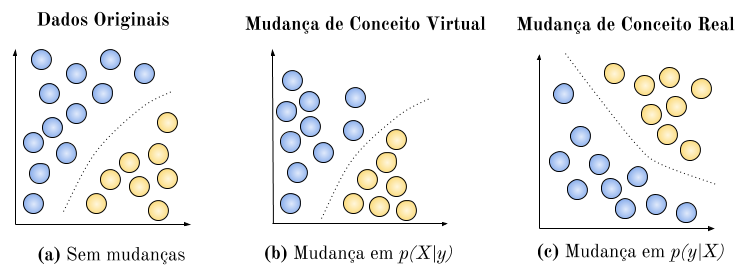
\includegraphics[scale=0.8]{imagens/concept_drift.png}
    \caption{Mudança de Conceito Virtual vs. Mudança de Conceito Real}
    \label{fig:real_and_virtual_concept_drift}
\end{center}
\end{figure}

Em \cite{Gama:2014:SCD:2597757.2523813}, o seguinte cenário é utilizado para explicar a diferença entre uma mudança de conceito real e uma virtual.
Considere um fluxo \textit{online} de anúncios do setor imobiliário.
Um usuário deseja classificar estes anúncios em relevantes e não relevantes.
Suponha, que à época, o usuário esteja buscando um novo apartamento. 
Isto torna anúncios de apartamentos residenciais relevantes, e anúncios de casa de férias irrelevantes.
Se o autor dos anúncios é alterado, o estilo de escrita sofre mudanças, mas os apartamentos permanecem relevantes para o usuário.
Este cenário corresponde a uma mudança de conceito virtual.
Considere que devido a uma crise, mais anúncios de apartamentos e menos de casas de férias aparecem, mas o editor dos anúncios permanece o mesmo.
Esta situação corresponde a uma mudança na probabilidade das classes.
Em outro cenário, assuma que o usuário acabou de comprar um apartamento e está em busca de um local para passar as férias.
Neste contexto, apartamentos tornaram-se irrelevantes e casas de férias, relevantes.
Apesar do editor dos anúncios e das probabilidades anteriores das classes permanecerem as mesmas, este cenário corresponde a uma mudança de conceito real.

Considerando apenas a perspectiva de predição, adaptações no modelo são necessárias apenas quando mudanças de conceito reais ocorrem, 
pois os limites de decisão do modelo corrente tornam-se obsoletos em relação aos novos exemplos \cite{Gama:2014:SCD:2597757.2523813}.
Adaptação, neste contexto, significa atualizar o modelo de decisão perante a nova distribuição dos dados a fim de manter uma alta acurácia.

Mudanças de conceito podem se apresentar sob diferentes padrões.
Conforme ilustrado na Figura \ref{fig:concept_drift_patterns}, mudanças de conceito podem ocorrer de forma abrupta, gradual, incremental ou recorrente.
 
\begin{figure}[!ht]
\begin{center}
    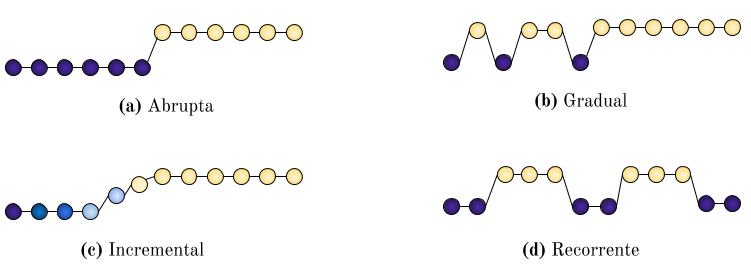
\includegraphics[scale=0.80]{imagens/concept_drift_patterns.png}
    \caption{Padrões de ocorrência de Mudanças de Conceito}
    \label{fig:concept_drift_patterns}
\end{center}
\end{figure}

Mudanças de conceito abruptas são alterações súbitas entre conceitos, como descrito na Figura \ref{fig:concept_drift_patterns} (a).
Por exemplo, o gênero literário de João pode subitamente mudar de ficção científica para auto-ajuda.
Outro exemplo, é a troca de um sensor por outro com diferente calibração, em uma planta industrial química \cite{Gama:2014:SCD:2597757.2523813}. 

Em constrate com a mudança de conceito abrupta, a mudança de conceito gradual significa uma transição mais lenta de um conceito para outro.
Isto é, durante a transição, são percebidos exemplos de ambos os conceitos.
Pode-se considerar que João, ao invés de subitamente passar a preferir livros de auto-ajuda, adquire interesse nestes ao longo do tempo.
Isto significa que João ainda tem interesse em livros de ficção científica, mas desenvolve, em paralelo, um crescente interesse por livros de auto-ajuda, que se tornará predominante.
A mudança de conceito gradual está representada na Figura \ref{fig:concept_drift_patterns} (b).

Mudanças de conceito incrementais apresentam diversos conceitos intermediários durante a transição de um conceito para outro.
No exemplo de João, é como se o seu interesse literário variasse de ficção científica para ficção científica e aventura, 
de ficção científica e aventura para aventura e suspense, de aventura e suspense para suspense e auto-ajuda, e finalmente de suspense e auto-ajuda para apenas auto-ajuda.
Considerando a planta industrial química e os sensores, seria como se um sensor perdesse precisão ao longo do tempo. 
A Figura \ref{fig:concept_drift_patterns} (c) demonstra a mudança de conceito incremental. 

Existe ainda outro padrão, denominado mudança de conceito recorrente \cite{Zliobaite:2010}. 
Conforme apresentado na Figura \ref{fig:concept_drift_patterns} (d), a mudança de conceito recorrente existe quando um conceito previamente ativo, 
reaparece após determinado período de tempo.
De volta ao nosso exemplo, João está atualmente interessado em livros de ficção científica.
Contudo, ele é presenteado com uma série de livros de auto-ajuda de um renomado autor brasileiro.
Após ler toda a série, João é premiado com descontos para livros de ficção científica.
Ele, volta, então, a ler livros de ficção científica comprados com os descontos recebidos.

É importante destacar que o fenômeno Mudança de Conceito tem sido estudado em diferentes comunidades de pesquisa, incluindo mineração de dados, 
aprendizado de máquina, estatística e recuperação de informação \cite{Zliobaite:2010}.
Contudo, o mesmo conceito pode ter diferentes nomeclaturas em cada comunidade.
Na Tabela \ref{tbl:taxonomy} são listados os termos correspondentes a Mudança de Conceito para cada área de pesquisa.

\begin{center} 
\begin{table}[!ht]
\label{tbl:taxonomy}
\begin{tabularx}{\textwidth}{|l|X|}
\cline{1-2}
\multicolumn{1}{|c|}{\textbf{Área}} & \multicolumn{1}{c|}{\textbf{Termos}}       \\ \cline{1-2}
Mineração de Dados                  & Mudança de Conceito                        \\ \cline{1-2}
Aprendizado de Máquina              & Mudança de Conceito, Mudança de Covariável \\ \cline{1-2}
Computação Evolucionária            & Ambiente Evolutivo, Ambiente em Mudança    \\ \cline{1-2}
IA e Robótica                       & Ambiente Dinâmico                          \\ \cline{1-2}
Estatísticas, Séries Temporais      & Não Estacionário                           \\ \cline{1-2}
Recuperação de Informação           & Evolução Temporal                          \\ \cline{1-2}
\end{tabularx}
\caption{Terminologia - Mudança de Conceito \cite{Zliobaite:2010}}
\end{table}
\end{center}

Outra possível fonte de equívoco é a utilização dos termos Detecção de \textit{Outliers}, Detecção de Novidade e Detecção de \textit{Change Points}.
Estes termos apresentam relação para com Detecção de Mudança de Conceito, pois dizem respeito a encontrar padrões que são diferentes dos padrões conhecidos.
Em alguns contextos, esses termos são usados indistitamente, entretanto, neste trabalho eles serão diferenciados.

De acordo com \cite{Chandola:2009:ADS:1541880.1541882}, 
detecção de \textit{outliers} refere-se a tarefa de encontrar padrões nos dados que não estão de acordo com o comportamento esperado.
Esses padrões podem ser denominados como: \textit{outliers}, anomalias, observações discordantes, exceções, peculiaridades ou aberrações.

Para \cite{Gama:2010:KDD:1855075}, exemplos esparsos e independentes, cujas características diferem muito daqueles que definem o modelo normal, 
devem ser considerados como \textit{outliers}, pois não há garantia de que representem um conceito. 
Em \cite{Aggarwal:2003:FCE:1315451.1315460}, os autores tipificam os \textit{outliers} como anomalias ou ruídos.
As anomalias constiuem um tipo especial de \textit{outlier}, que é de interesse dos analistas.
Contudo, conforme \cite{Gama:2010:KDD:1855075}, é necessário um grupo conciso de exemplos para evidenciar o aparecimento de um novo conceito, ou novidade.

Segundo \cite{Chandola:2009:ADS:1541880.1541882}, a Detecção de Novidade objetiva detectar padrões não observados (emergentes) nos dados.
Entretanto, esse termo se distingue da detecção de \textit{outliers}, pois os novos padrões, geralmente, são incorporados ao modelo normal.
Apesar de apresentarem definições próximas, a Detecção de Mudança de Conceito engloba a Detecção de Novidade e a extrapola, ao identificar 
mudanças de conceito reais a partir do \textit{feedback} sobre a performance preditiva \cite{Gama:2010:KDD:1855075}.

Técnicas para Detecção de \textit{Change Points} identificam variações abruptas de valor em séries temporais, que podem representar transições entre estados.
Diferenciam-se das técnicas para Detecção de Mudança de Conceito pois são aplicadas em séries temporais unidimensionais estacionárias \cite{Aminikhanghahi:2017:SMT:3086013.3086037}.

Na seção seguinte, serão detalhados os principais algoritmos para Detecção de Mudança de Conceito, 
priorizando algoritmos que não dependem de \textit{feedback} da performance preditiva (correta rotulação dos exemplos).

\subsection{Algoritmos para Detecção de Mudança de Conceito}

Os algoritmos para Detecção de Mudança de Conceito são os responsáveis pela identificação, de forma explícita, das mudanças de conceito em fluxos de dados \cite{Gama:2014:SCD:2597757.2523813}.
Estes métodos caracterizam e quantificam as mudanças de conceito através da delimitação dos instantes ou intervalos de tempo em que as mudanças ocorreram \cite{Basseville:1993:DAC:151741}.

As técnicas propostas na literatura podem ser divididas em duas categorias, baseado na dependência ou não de dados rotulados:
\begin{description}
    \item[Algoritmos Explícitos/Supervisionados] Dependem da rotulação dos dados por um especialista.
    Estes rótulos são utilizados no cálculo de métricas de performance como acurácia e taxa de erro, que são monitoradas ao longo do tempo.
    Mudanças de conceito são sinalizadas quando o algoritmo detecta que essas métricas atingiram um limite previamente definido.

    \item[Algoritmos Implícitos/Não Supervisionados] Independem da rotulação por especialistas, 
    baseando-se em propriedades dos valores dos exemplos, para sinalizar desvios.
    São mais propensos a alarmes falsos, mas a independência de rótulos os torna interessantes para contextos onde a obtenção de rótulos é dispendiosa, demorada ou inviável.
\end{description}

Em sua pesquisa \cite{Gama:2014:SCD:2597757.2523813} categorizou os algoritmos supervisionados em três grupos principais:

\begin{description}
    \item[Métodos Baseados em Análise Sequencial] Avaliam, de forma sequenciada, os resultados das predições conforme tornam-se disponíveis (taxa de erro).
    Indicam a ocorrência de mudança de conceito quando um limite pré-definido é atingido.
    Os algoritmos \textit{Cumulative Sum (CUSUM)}, \textit{PageHinkley (PH)} \cite{Page:CUSUM:PageHinkley:1954} e \textit{Geometric Moving Average (GMA)} \cite{Roberts:2000:CCT:338441.338464}
    são representantes deste grupo.

    \item[Abordagens baseadas em Estatística] Identificam mudanças de conceito através da análise de parâmetros estatísticos como média e desvio padrão para os resultados das predições.
    Os métodos \textit{Drift Detection Method (DDM)} \cite{GamaMCR04}, 
    \textit{Early Drift Detection Method (EDDM)} \cite{EDDM}, 
    \textit{Exponentially Weighted Moving Average (EWMA)} \cite{Ross:2012:EWM:2076039.2076307} e 
    \textit{Reactive Drift Detection Method (RDDM)} \cite{Barros:RDDM:2017} são exemplos deste grupo.

    \item[Métodos baseados em Janelas] Geralmente, utilizam uma janela de tamanho fixo para sumarizar informações passadas e uma janela deslizante para sumarizar dados mais recentes.
    A mudança de conceito é detectada quando há uma diferença significativa entre as distribuições das janelas.
    Esta diferença é detectada a partir de testes estatísticos ou desigualdades matemáticas, considerando como hipótese nula a igualdade entre as distribuições.
    Os algoritmos 
    \textit{Adaptive Windowing (ADWIN)} \cite{BifetG07}, 
    \textit{SeqDrift} \cite{PearsSK14:SeqDrift:2014}, 
    \textit{HDDMA} e \textit{HDDMW} \cite{BlancoCRBDM15:HDDMA:HDDMW:2015}
    são membros desta família.
\end{description}

Os algoritmos implícitos também foram divididos em três grupos \cite{GONCALVES20148144}:

\begin{description}
    \item[Detecção de Novidade / Métodos de Agrupamento] 
    Utilizam a distância e/ou a densidade dos dados para detectar novos padrões.
    O algoritmo identifica exemplos suspeitos e os atribui a uma classe \textit{Desconhecido}, indicando a necessidade de uma avaliação adicional.
    As técnicas de agrupamento e detecção de \textit{outliers} são estratégias de implementação populares para estes algoritmos, 
    pois sintetizam os dados correntes e aplicam medidas de dissimilaridade para identificar novos padrões \cite{Ryu:Kantardzic:2012}.
    Os métodos 
    \textit{OLINDDA} \cite{Spinosa:2007:OCA:1244002.1244107},
    \textit{MINAS} \cite{Faria:2013:NDA:2480362.2480515},
    \textit{Woo} \cite{Ryu:Kantardzic:2012},
    \textit{DETECTNOD} \cite{Hashemi:Hayat:DETECTNOD:2010},
    \textit{ECSMiner} \cite{Masud:2011:CNC:1978259.1978529} e
    \textit{GC3} \cite{Sethi2016b:GC3} fazem parte deste grupo.
    
    \item[Monitoramento de distribuição multivariada]
    Monitoram diretamente a distribuição dos dados, considerando cada atributo.
    Este monitoramento é feito através de subconjuntos dos dados.
    Um subconjunto de treinamento tem sua distribuição sumarizada e armazenada, sendo utilizada como referência.
    A distribuição referência é comparada à distribuição do subconjunto atual, e havendo diferenças significativas, a mudança de conceito é sinalizada.
    Os algoritmos
    \textit{CoC} \cite{Lee:Magoules:CoC:2012},
    \textit{HDDDM} \cite{Ditzler:Polikar:HDDDM:2011},
    \textit{PCA-detect} \cite{Kuncheva:PCADetect:20085}
    são representantes deste grupo.

    \item[Monitoramento dependente de modelo]
    As técnicas elencadas nos grupos anteriores monitoram desvios na distribuição dos dados, considerando cada atributo.
    Essencialmente, esses métodos assumem que alterações na distribuição $P(X)$ implicarão mudanças na performance do classificador $P(Y|X)$.
    Apesar de permitir a aplicação de qualquer tipo de classificador, essa presunção leva a uma maior quantidade de falsos alarmes.
    As técnicas dependentes de modelo restringem-se aos classificadores probabilísticos e monitoram as probabilidades a posteriori destes, 
    para detecção de mudanças de conceito \cite{Zliobaite:2010}.
    A utilização das probabilidades a posteriori diminui a incidência de falsos alarmes e torna o processo computacionalmente eficiente, 
    pois apenas um único fluxo univariado de valores é observado.
    Os métodos 
    \textit{A-distance} \cite{Dredze:ADistance:2010585},
    \textit{CDBD} \cite{Lindstrom:CDBD:2013} e
    \textit{Margin} \cite{Dries:Margin:2009} participam deste grupo.
\end{description}

Por fim, a Tabela \ref{tbl:abordagens} sumariza as categorias, os grupos e as respectivas técnicas mencionadas nesta seção.

% Please add the following required packages to your document preamble:
% \usepackage{graphicx}
\begin{table}[!ht]
    \centering
    \resizebox{\textwidth}{!}{%
    \begin{tabular}[t]{@{}lllll@{}}
    \hline \\
    Algoritmos Explícitos/Supervisionados     & Métodos Baseados em Análise Sequencial        & \begin{tabular}[t]{@{}l@{}} Cumulative Sum (CUSUM) \\ PageHinkley (PH) \cite{Page:CUSUM:PageHinkley:1954} \\ Geometric Moving Average (GMA) \cite{Roberts:2000:CCT:338441.338464}\end{tabular}                                                                                                                        &  &  \\ \\
                                              & Abordagens baseadas em Estatística            & \begin{tabular}[t]{@{}l@{}} Drift Detection Method (DDM) \cite{GamaMCR04} \\  Early Drift Detection Method (EDDM) \cite{EDDM} \\  Exponentially Weighted Moving Average (EWMA) \cite{Ross:2012:EWM:2076039.2076307} \\ Reactive Drift Detection Method (RDDM) \cite{Barros:RDDM:2017} \end{tabular}                                                                &  &  \\ \\
                                              & Métodos baseados em Janelas                   & \begin{tabular}[t]{@{}l@{}} Adaptive Windowing (ADWIN) \cite{BifetG07} \\   SeqDrift \cite{PearsSK14:SeqDrift:2014} \\   HDDMA/HDDMW \cite{BlancoCRBDM15:HDDMA:HDDMW:2015} \end{tabular}                                                                                            &  &  \\ \\
    
    Algoritmos Implícitos/Não Supervisionados & Detecção de Novidade / Métodos de Agrupamento & \begin{tabular}[t]{@{}l@{}} OLINDDA \cite{Spinosa:2007:OCA:1244002.1244107} \\   MINAS \cite{Faria:2013:NDA:2480362.2480515} \\   Woo \cite{Ryu:Kantardzic:2012} \\   DETECTNOD \cite{Hashemi:Hayat:DETECTNOD:2010} \\   ECSMiner \cite{Masud:2011:CNC:1978259.1978529} \\   GC3 \cite{Sethi2016b:GC3} \end{tabular} &  &  \\ \\
                                              & Monitoramento de distribuição multivariada    & \begin{tabular}[t]{@{}l@{}} CoC \cite{Lee:Magoules:CoC:2012} \\ HDDDM \cite{Ditzler:Polikar:HDDDM:2011} \\ PCA-detect \cite{Kuncheva:PCADetect:20085} \end{tabular}                                       &  &  \\ \\
                                              & Monitoramento dependente de modelo            & \begin{tabular}[t]{@{}l@{}} A-distance \cite{Dredze:ADistance:2010585} \\ CDBD \cite{Lindstrom:CDBD:2013} \\ Margin \cite{Dries:Margin:2009} \end{tabular}                                                                                        &  &  \\ \\
    \hline
    \end{tabular}%
    }
    \caption{Sumário - Abordagens de detecção \cite{Sethi:2017:RDC:3096751.3096864}}
    \label{tbl:abordagens}
\end{table}

\subsection{Ferramentas}

Nesta seção, os frameworks \textit{Massive Online Analysis} (MOA) e \textit{Tornado} serão apresentados.
Estes frameworks possibilitam a implementação e a análise - perante o estado da arte - de algoritmos para detecção de mudança de conceito.
Ambos permitem a avaliação entre técnicas, utilizando diferentes \textit{datasets}.

\subsection{MOA}

O MOA divide suas funcionalidades em tarefas (\textit{tasks}).
As principais tarefas incluem:
treino de classificadores,
avaliação de modelos e 
produção de fluxos de dados.
Tarefas podem ser executadas a partir de uma interface gráfica (GUI) ou por linha de comando.
A tela principal da aplicação é demonstrada na Figura \ref{fig:moa}.
A interface gráfica da aplicação permite executar múltiplas tarefas de forma concorrente, 
possibilitando o controle de execução e a visualização de resultados parciais.

\begin{figure}[!ht]
\begin{center}
    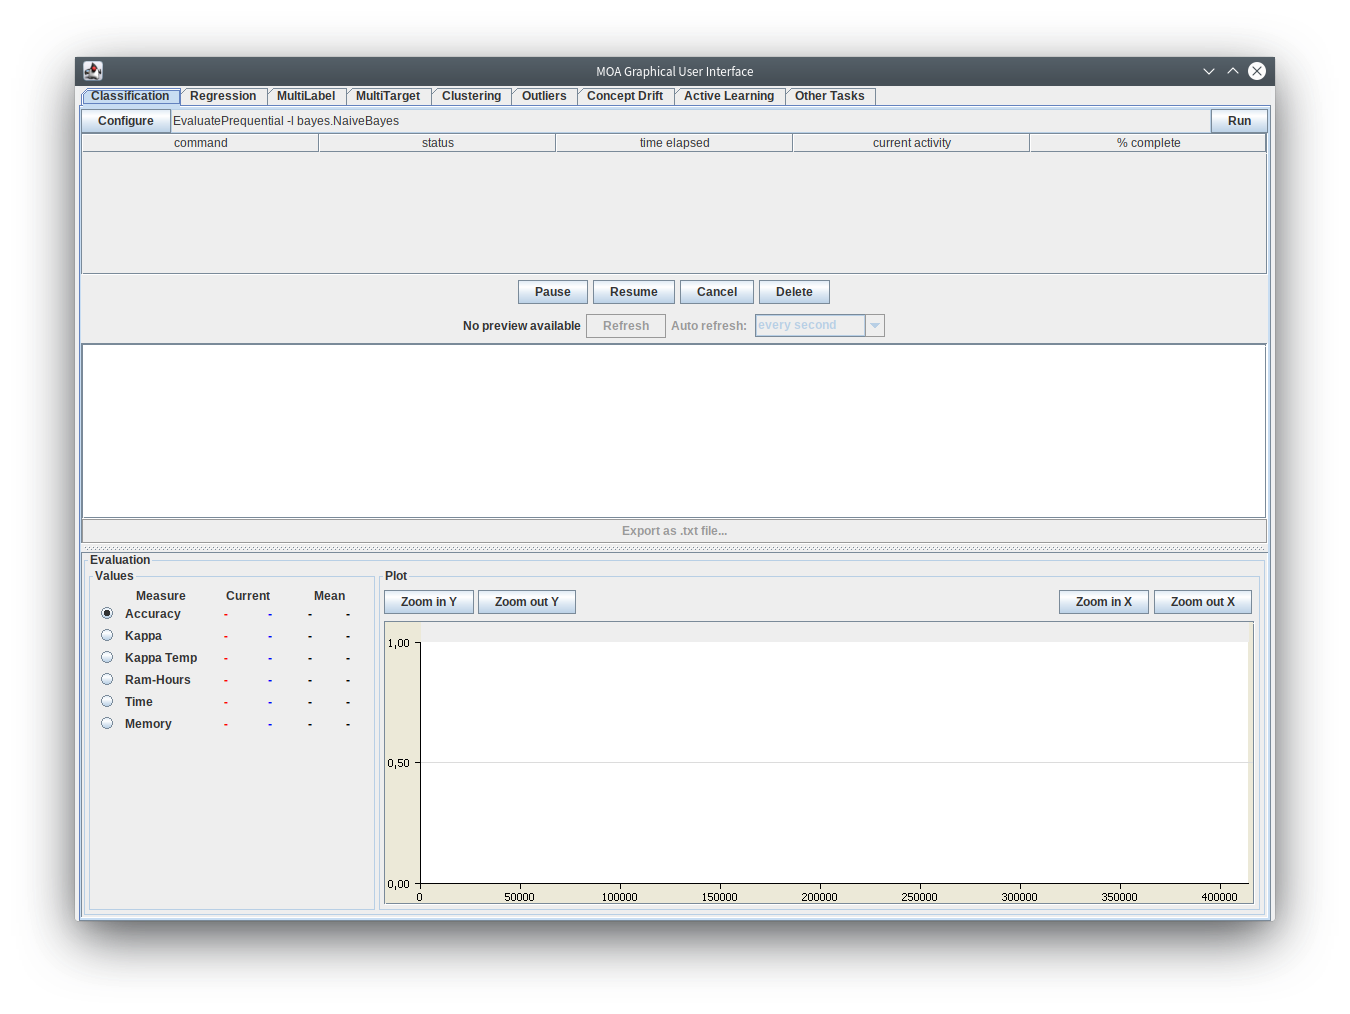
\includegraphics[scale=0.5]{imagens/moa.png}
    \caption{MOA - Tela Inicial}
    \label{fig:moa}
\end{center}
\end{figure}

O MOA é capaz de ler arquivos \textit{ARFF}, popularizados na área de aprendizado de máquina por serem utilizados no projeto WEKA \cite{Hall:2009:WDM:1656274.1656278}.
A ferramenta também permite a produção de fluxos de dados dinamicamente através de geradores, unindo diferentes fluxos ou aplicando filtros a fluxos existentes.
Alguns dos geradores de fluxo disponíveis no MOA são:
\textit{Random Trees} \cite{Domingos:2000:MHD:347090.347107}
\textit{SEA} \cite{Street:2001:SEA:502512.502568}, 
\textit{STAGGER} \cite{Schlimmer1986}, 
\textit{Rotating Hyperplane} \cite{Wang:2003:MCD:956750.956778},
\textit{Random RBF}, 
\textit{LED} \cite{Gama:2003:ADT:956750.956813}, 
\textit{Waveform} \cite{Gama:2003:ADT:956750.956813}, 
 e \textit{Function} \cite{Jin:2003:EDT:956750.956821}.

\subsection{Tornado}
\blindtext

\section{Redes de Função de Base Radial}
\blindtext
  
\section{Trabalhos Relacionados}
\blindtext

\section{Considerações Finais}
\blindtext

\xchapter{Plano de Pesquisa}{} \label{plano_pesquisa}
\section{Considerações Iniciais}
\blindtext

\section{Descrição do Problema}
\blindtext

\subsection{Atividades de Pesquisa}
\blindtext

\section{Considerações Finais}
\blindtext

\xchapter{Experimentos Iniciais}{} \label{experimentos_iniciais}
\section{Considerações Iniciais}
\blindtext

\section{Configuração dos Experimentos}
\blindtext

\section{Método de Pettitt}
\blindtext

\section{Redes de Função de Base Radial}
\blindtext

\section{Considerações Finais}
\blindtext


%% Parte pos-textual
\backmatter

% Bibliografia
% É aconselhável utilizar o BibTeX a partir de um arquivo, digamos "biblio.bib".
% Para ajuda na criação do arquivo .bib e utilização do BibTeX, recorra ao
% BibTeXpress em www.cin.ufpe.br/~paguso/bibtexpress
\bibliographystyle{abntex2-alf}
\bibliography{biblio}

% Apendices
% Comente se naoo houver apendices
%\appendix

%\xchapter{Exemplo de Ap\^endice}{} %sem preambulo
%\lipsum
% Eh aconselhavel criar cada apendice em um arquivo separado, digamos
% "apendice1.tex", "apendice.tex", ... "apendiceM.tex" e depois
% inclui--los com:
%\xchapter{Decomposição das séries temporais}{} %sem preambulo
\label{apendice1}
\section{Considerações Iniciais}
Neste apêndice consta as 40 séries temporais utilizadas nos experimentos mostrados no Capitulo \ref{experimentos}. As séries foram divididas em 4 tipos conforme a Tabela \ref{series}, onde o tipo representa um conjunto de 10 séries senoide ou cossenoide, sendo acrescida de ruído ou acrescida de ruído e tendência.
Nas imagens são representadas, a séries original,   seu componente determinístico e seu componente estocástico, os quais foram extraídos após a decomposição.
\section{Séries TIPO 1}
10 séries cossenoide com ruído ao longo da série.
\graphicspath{{imagens/}}
\begin{figure}[H]
\begin{center}
  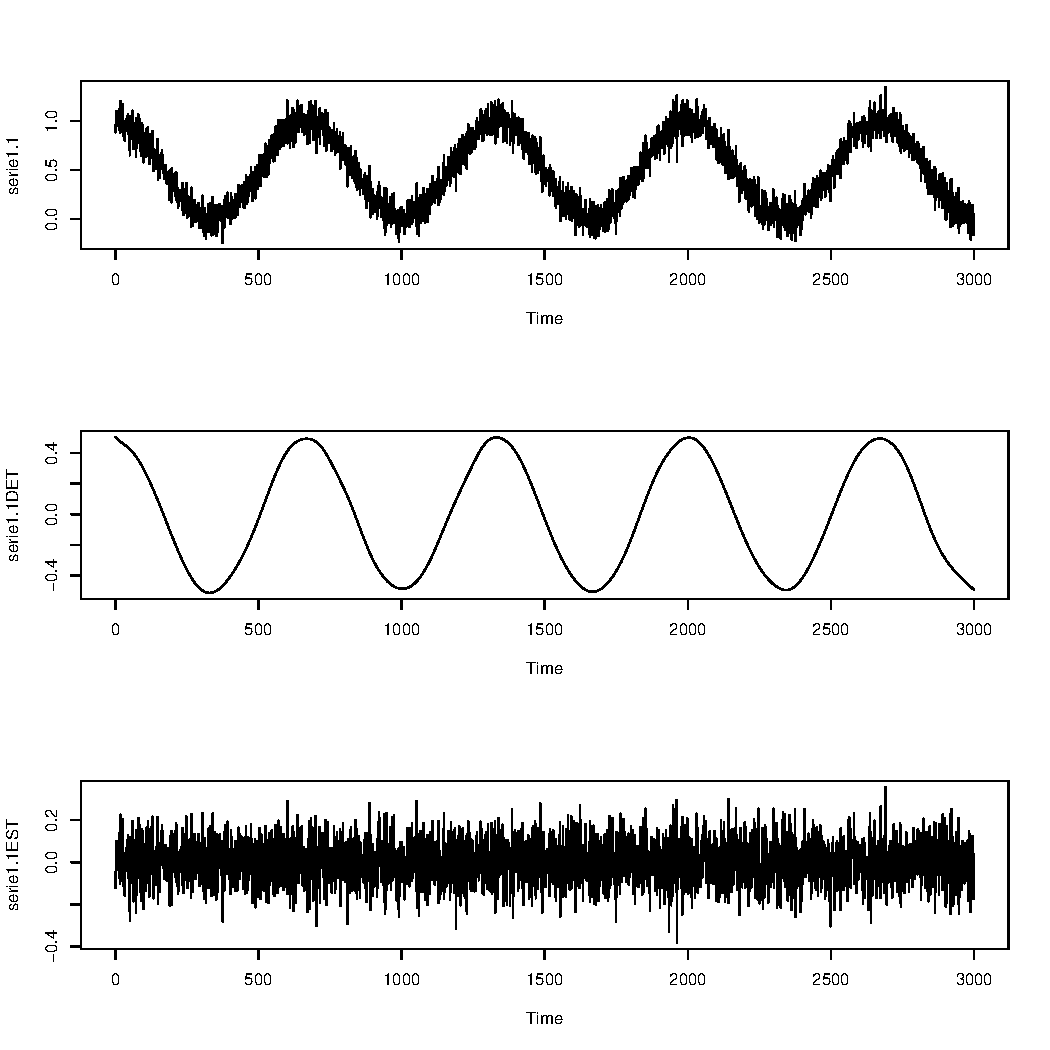
\includegraphics[scale=0.43]{serie1_1.pdf} \quad
  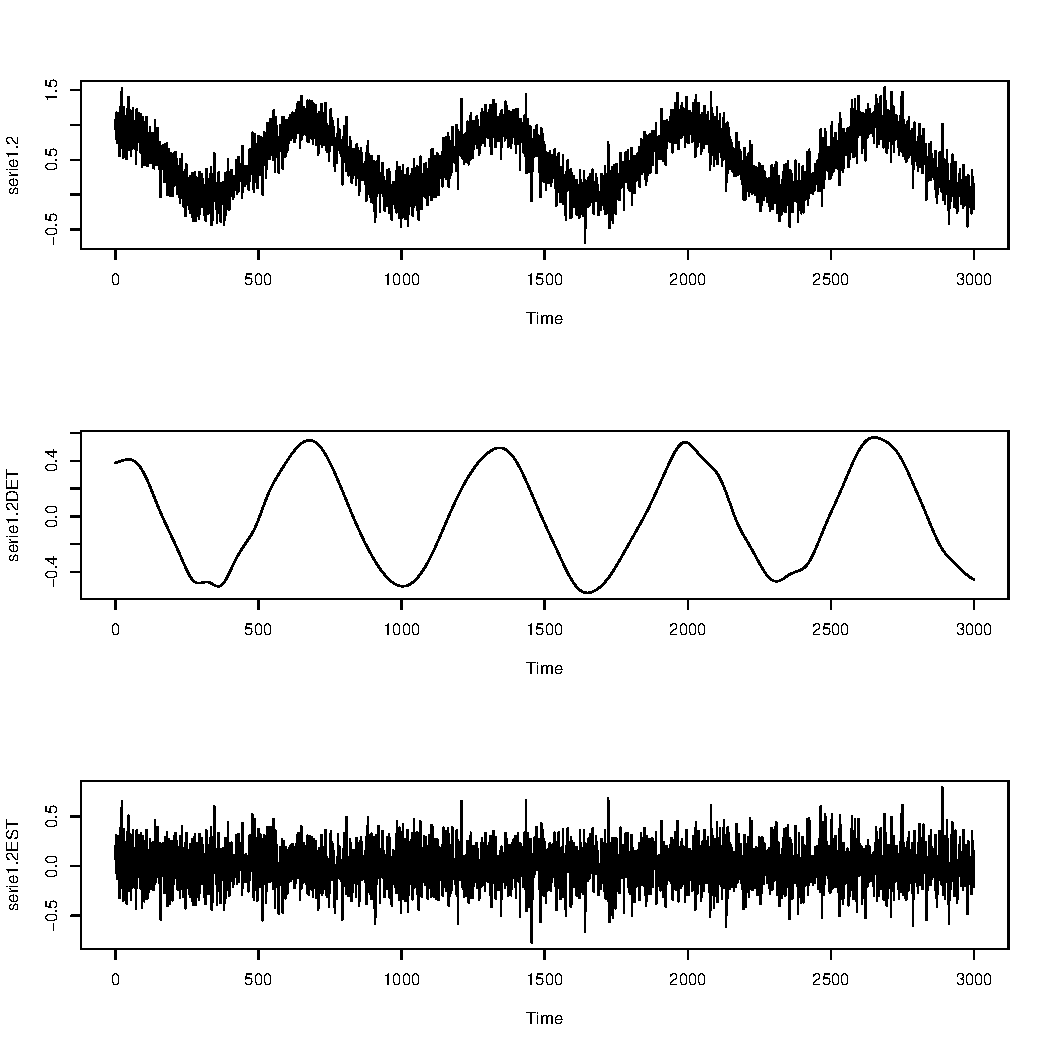
\includegraphics[scale=0.43]{serie1_2.pdf}
  \caption{Série 1.1 e Série 1.2}

\end{center}
\end{figure}

\graphicspath{{imagens/}}
\begin{figure}[H]
\begin{center}
  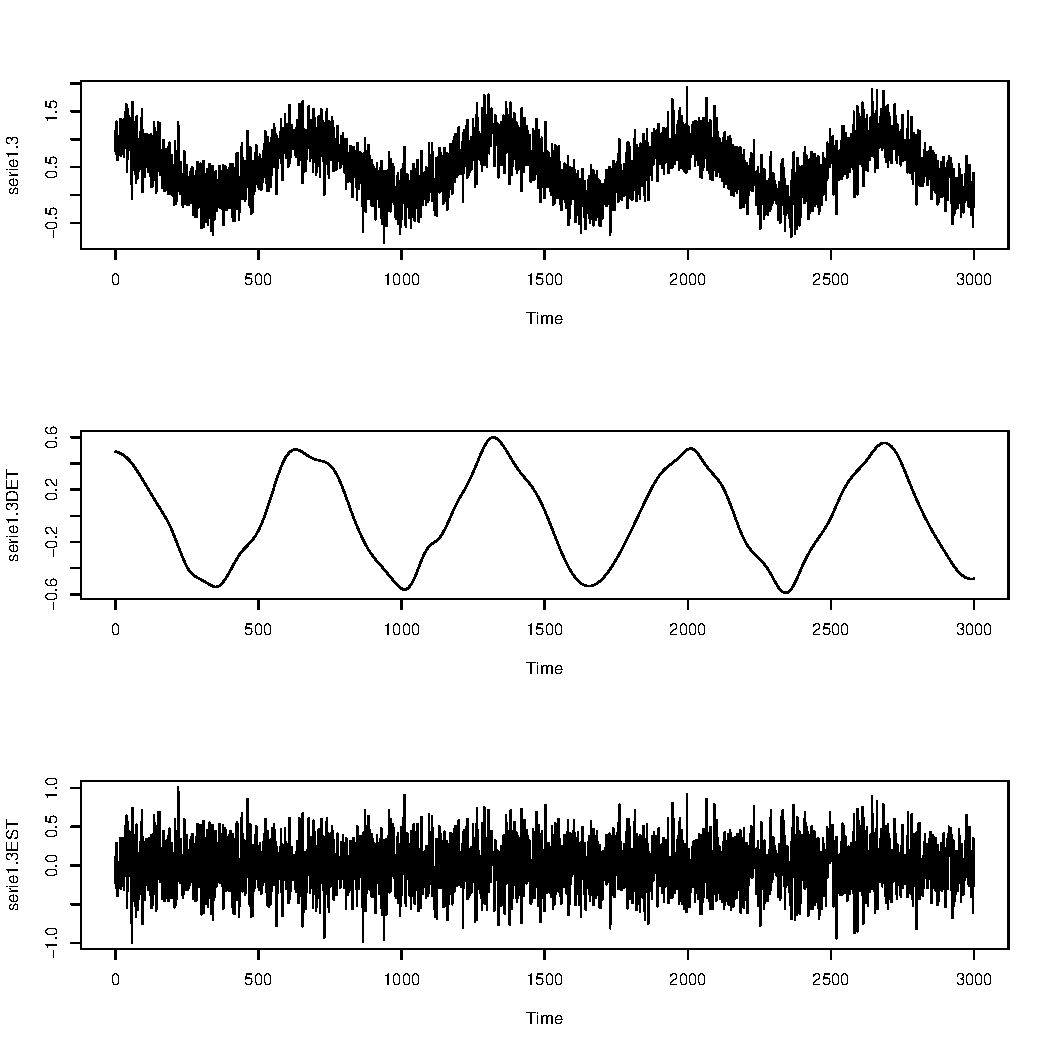
\includegraphics[scale=0.43]{serie1_3.pdf} \quad
  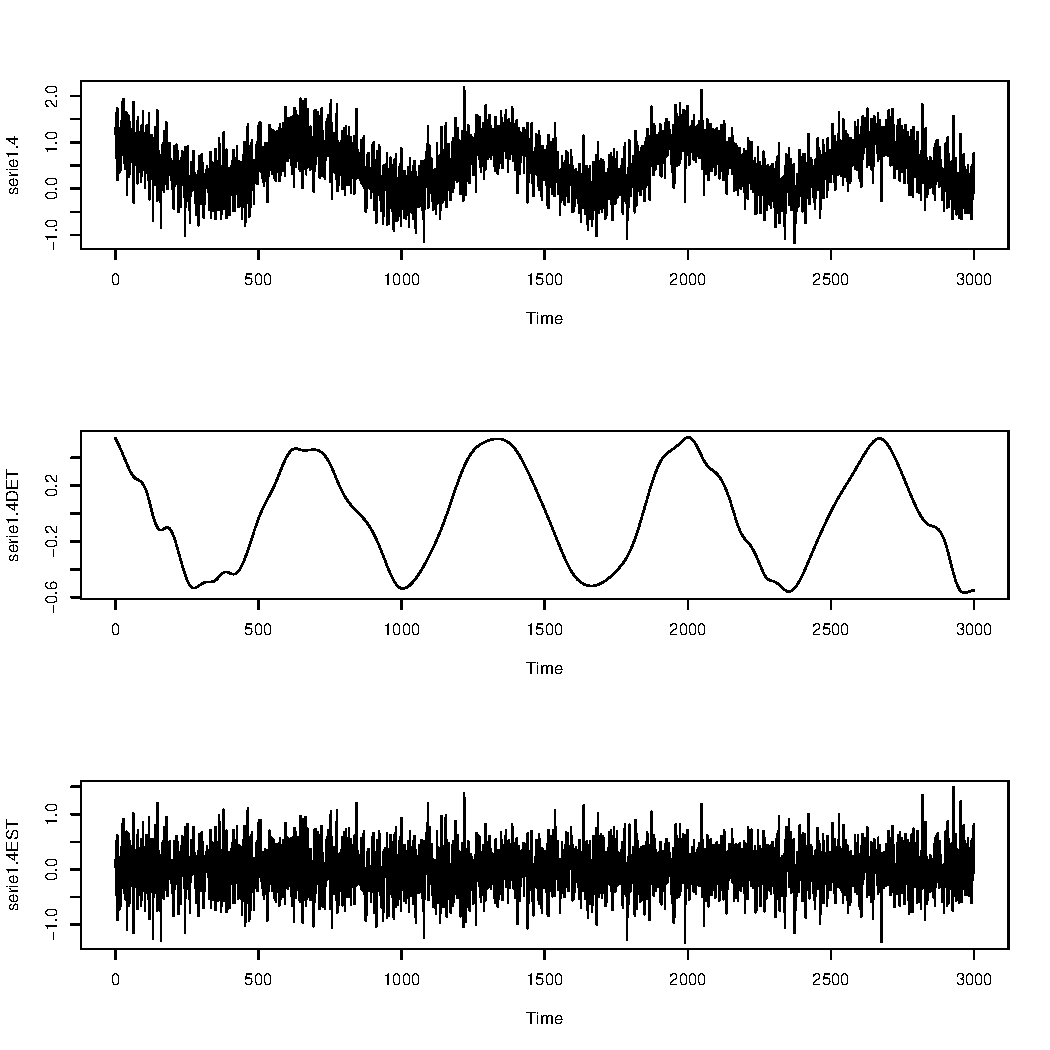
\includegraphics[scale=0.43]{serie1_4.pdf}
  \caption{Série 1.3 e Série 1.4}

\end{center}
\end{figure}

\graphicspath{{imagens/}}
\begin{figure}[H]
\begin{center}
  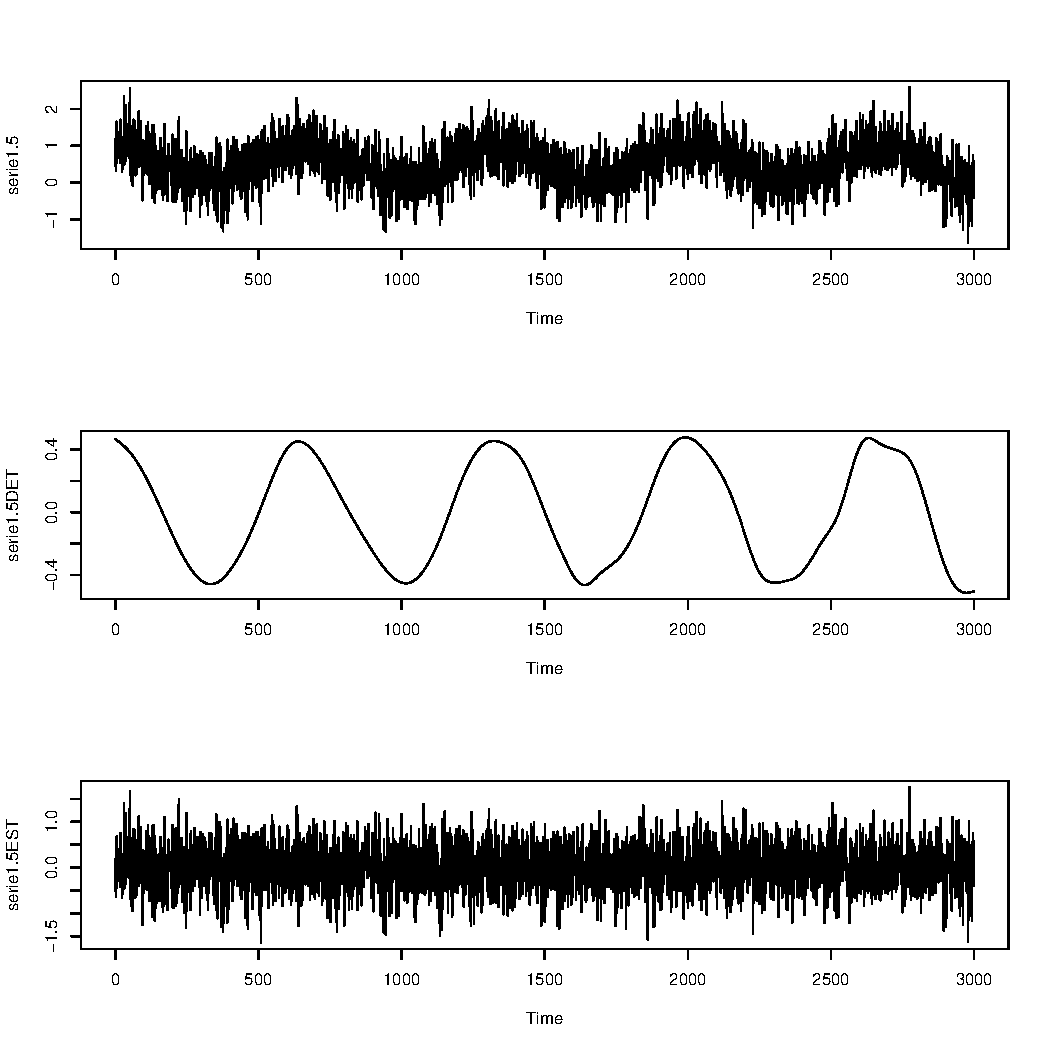
\includegraphics[scale=0.43]{serie1_5.pdf} \quad
  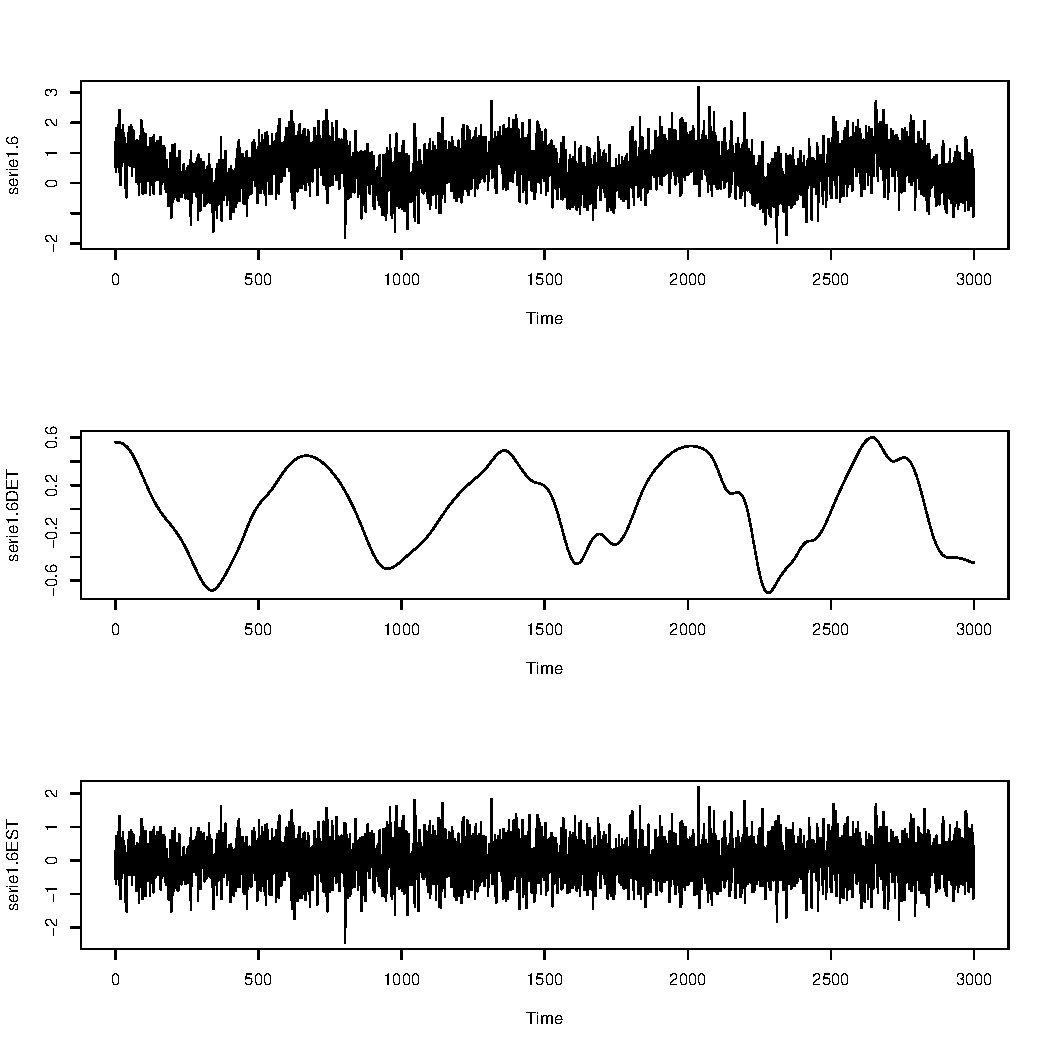
\includegraphics[scale=0.43]{serie1_6.pdf}
  \caption{Série 1.5 e Série 1.6}

\end{center}
\end{figure}

\graphicspath{{imagens/}}
\begin{figure}[H]
\begin{center}
  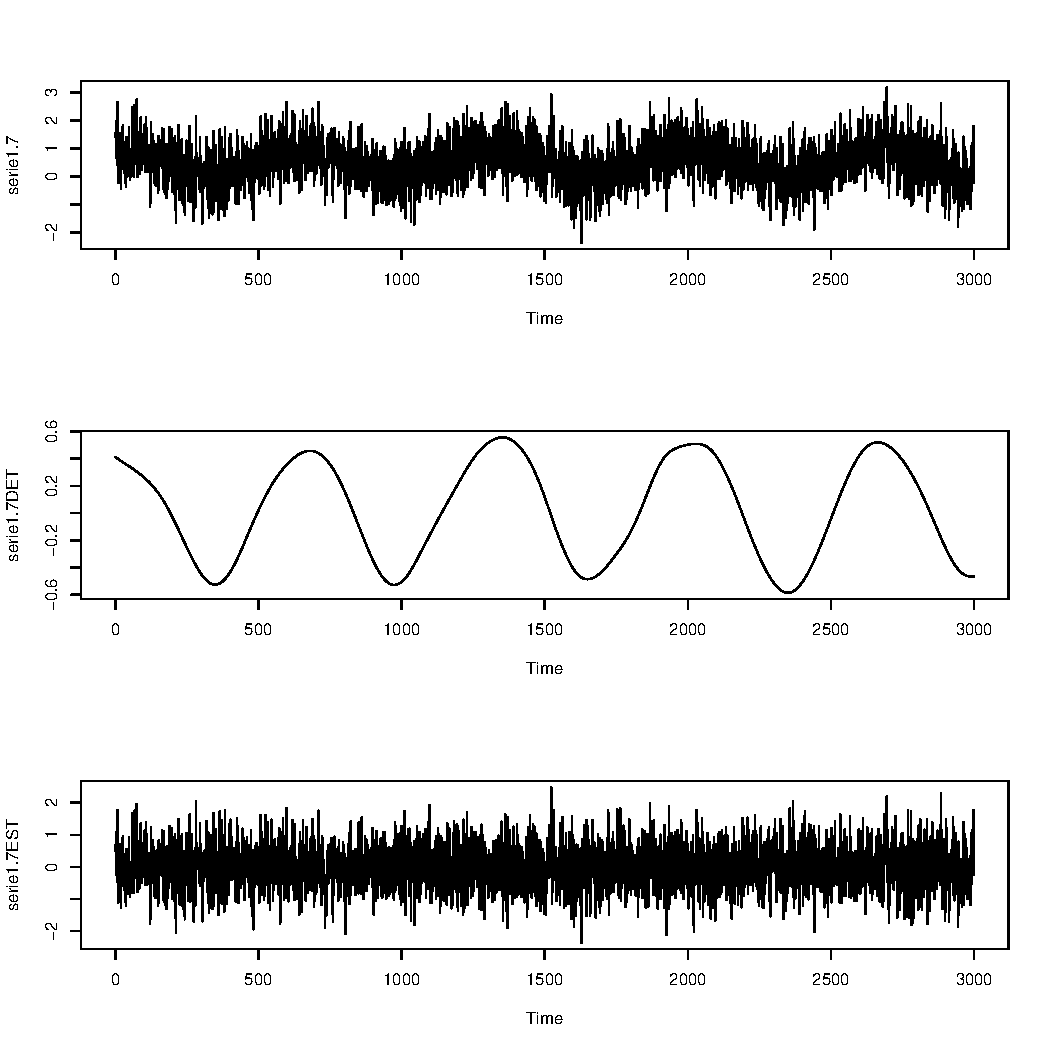
\includegraphics[scale=0.43]{serie1_7.pdf} \quad
  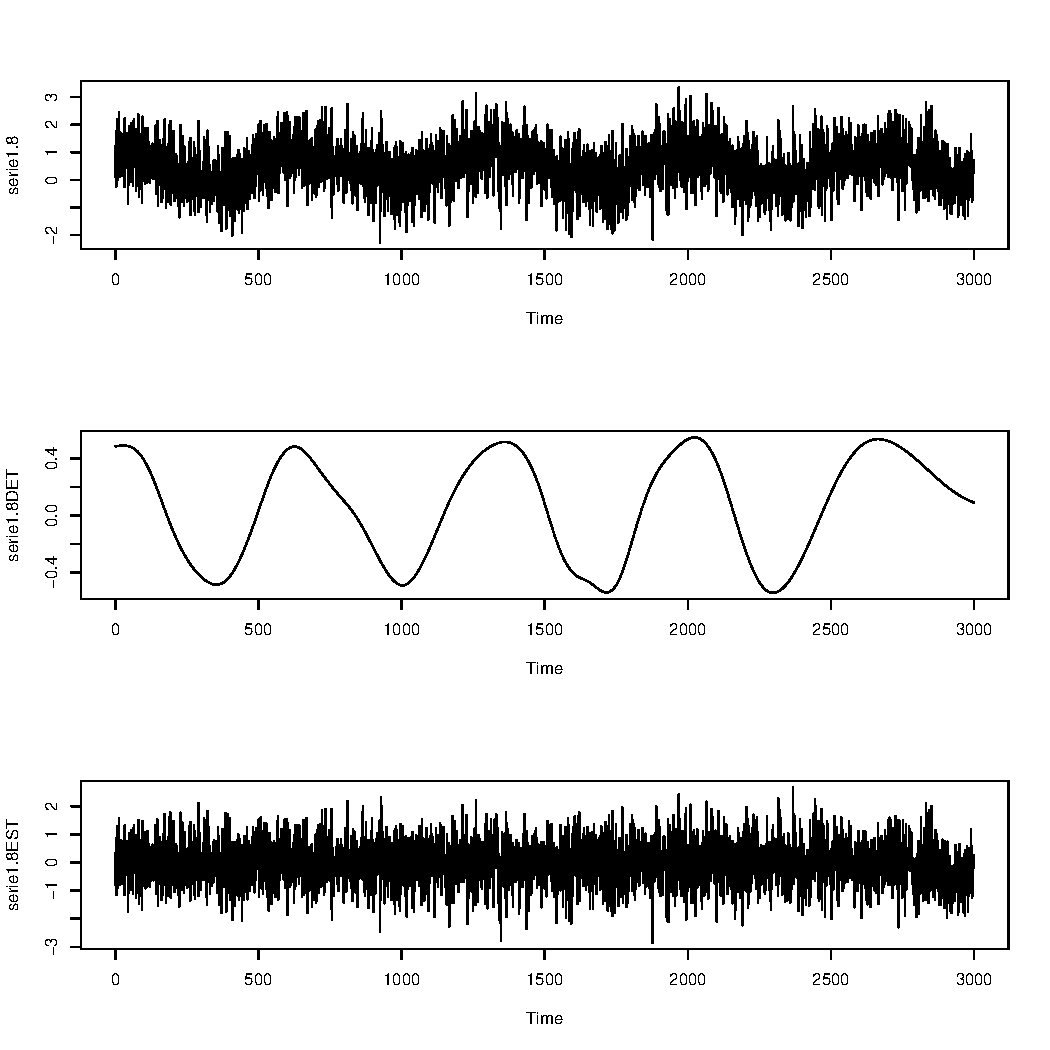
\includegraphics[scale=0.43]{serie1_8.pdf}
  \caption{Série 1.7 e Série 1.8}

\end{center}
\end{figure}

\graphicspath{{imagens/}}
\begin{figure}[H]
\begin{center}
  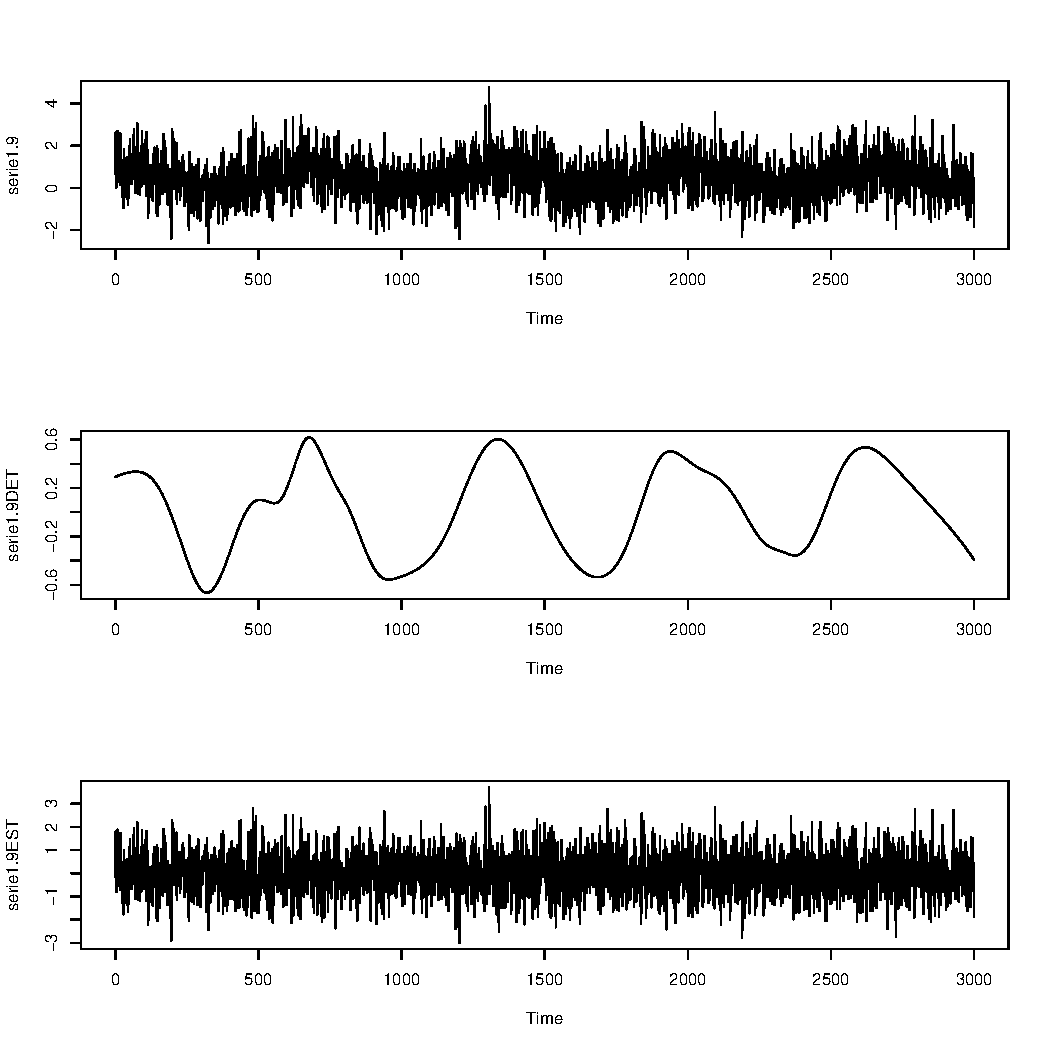
\includegraphics[scale=0.43]{serie1_9.pdf} \quad
  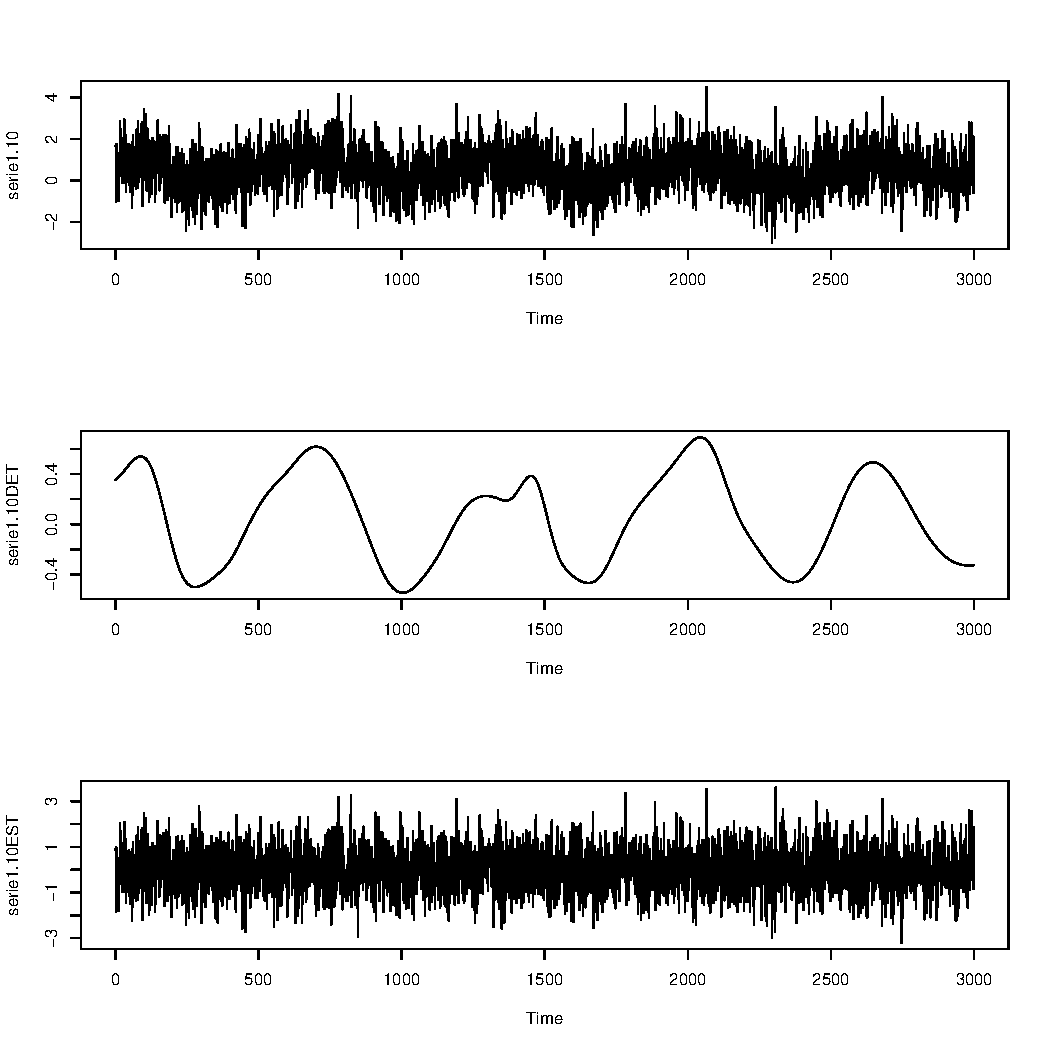
\includegraphics[scale=0.43]{serie1_10.pdf}
  \caption{Série 1.9 e Série 1.10}

\end{center}
\end{figure}

\section{Séries TIPO 2}
10 séries cossenoide com ruído ao longo da série e tendência.
\graphicspath{{imagens/}}
\begin{figure}[H]
\begin{center}
  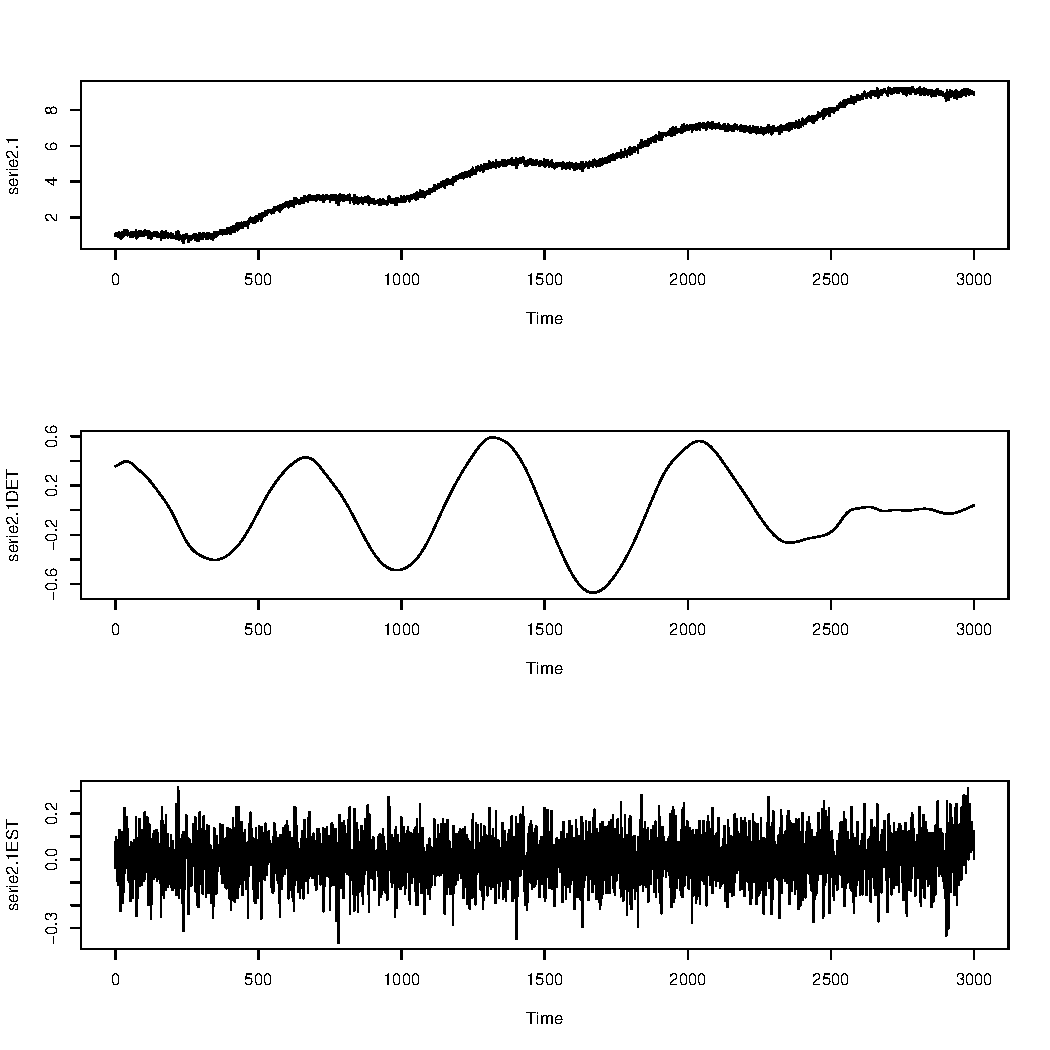
\includegraphics[scale=0.43]{serie2_1.pdf} \quad
  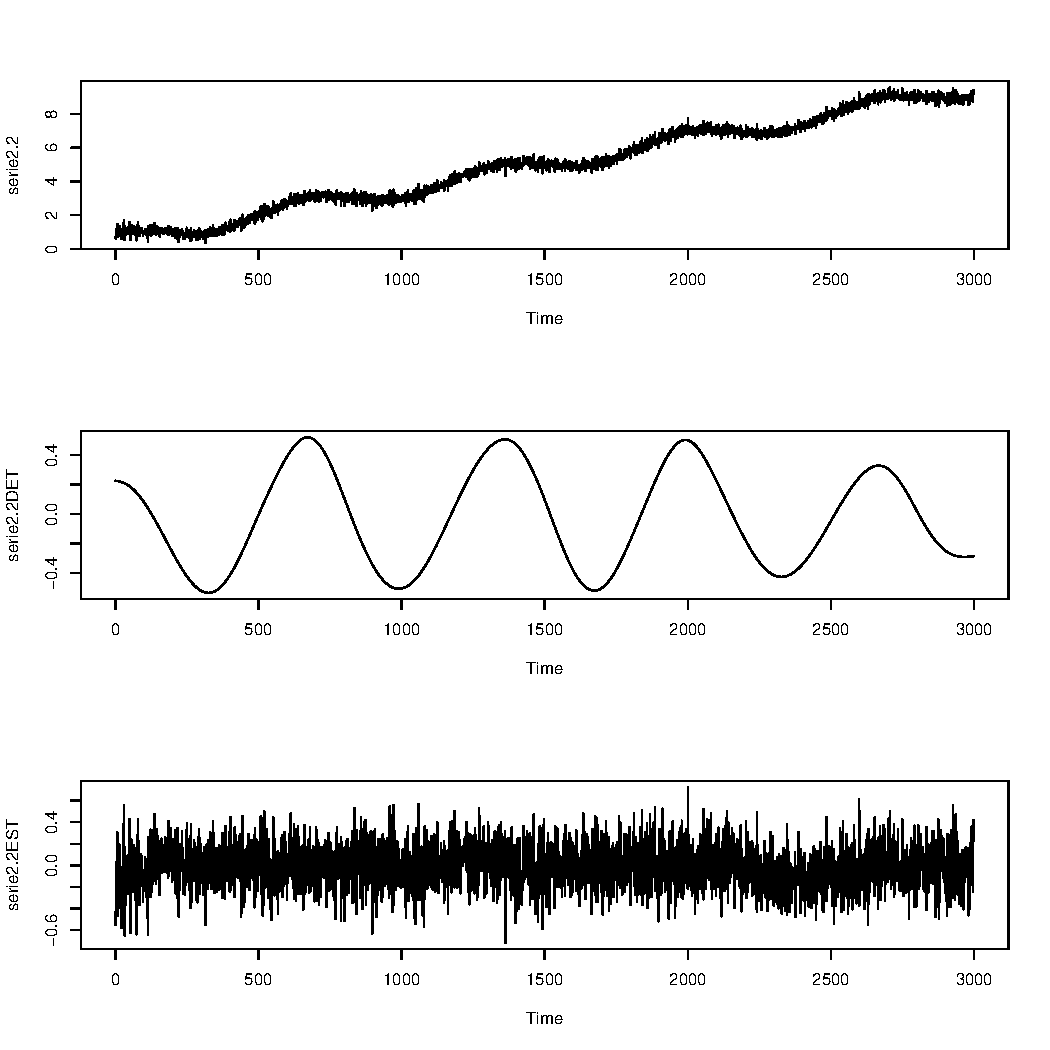
\includegraphics[scale=0.43]{serie2_2.pdf}
  \caption{Série 2.1 e Série 2.2}

\end{center}
\end{figure}

\graphicspath{{imagens/}}
\begin{figure}[H]
\begin{center}
  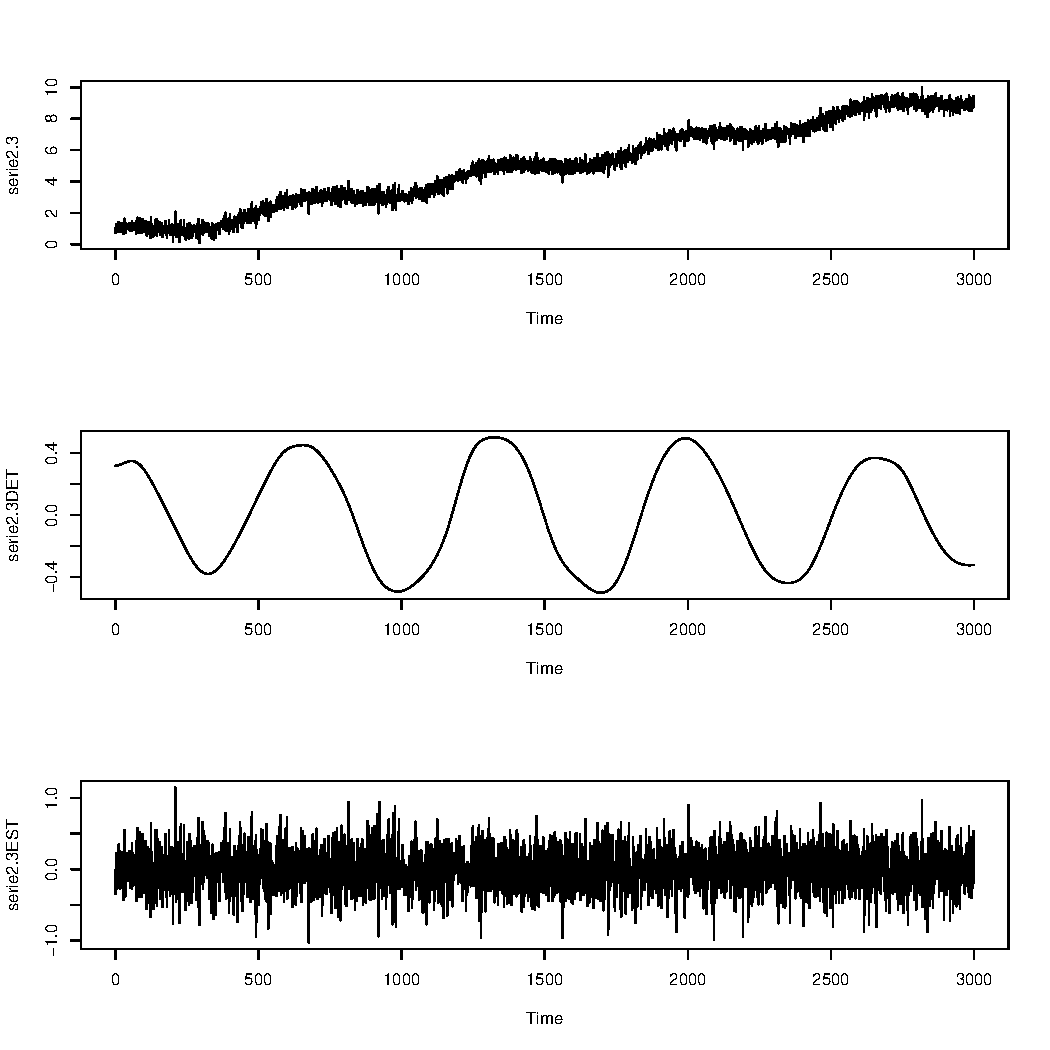
\includegraphics[scale=0.43]{serie2_3.pdf} \quad
  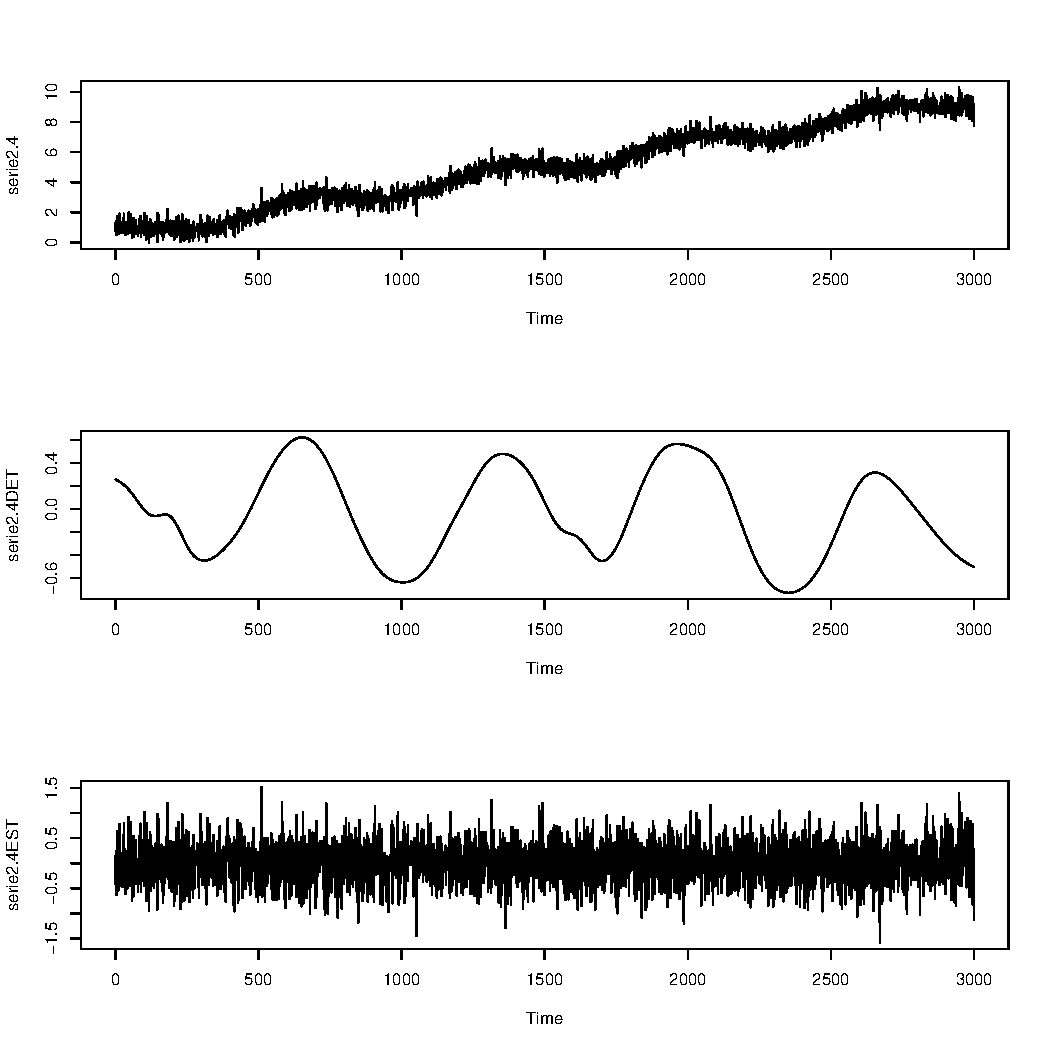
\includegraphics[scale=0.43]{serie2_4.pdf}
  \caption{Série 2.3 e Série 2.4}

\end{center}
\end{figure}

\graphicspath{{imagens/}}
\begin{figure}[H]
\begin{center}
  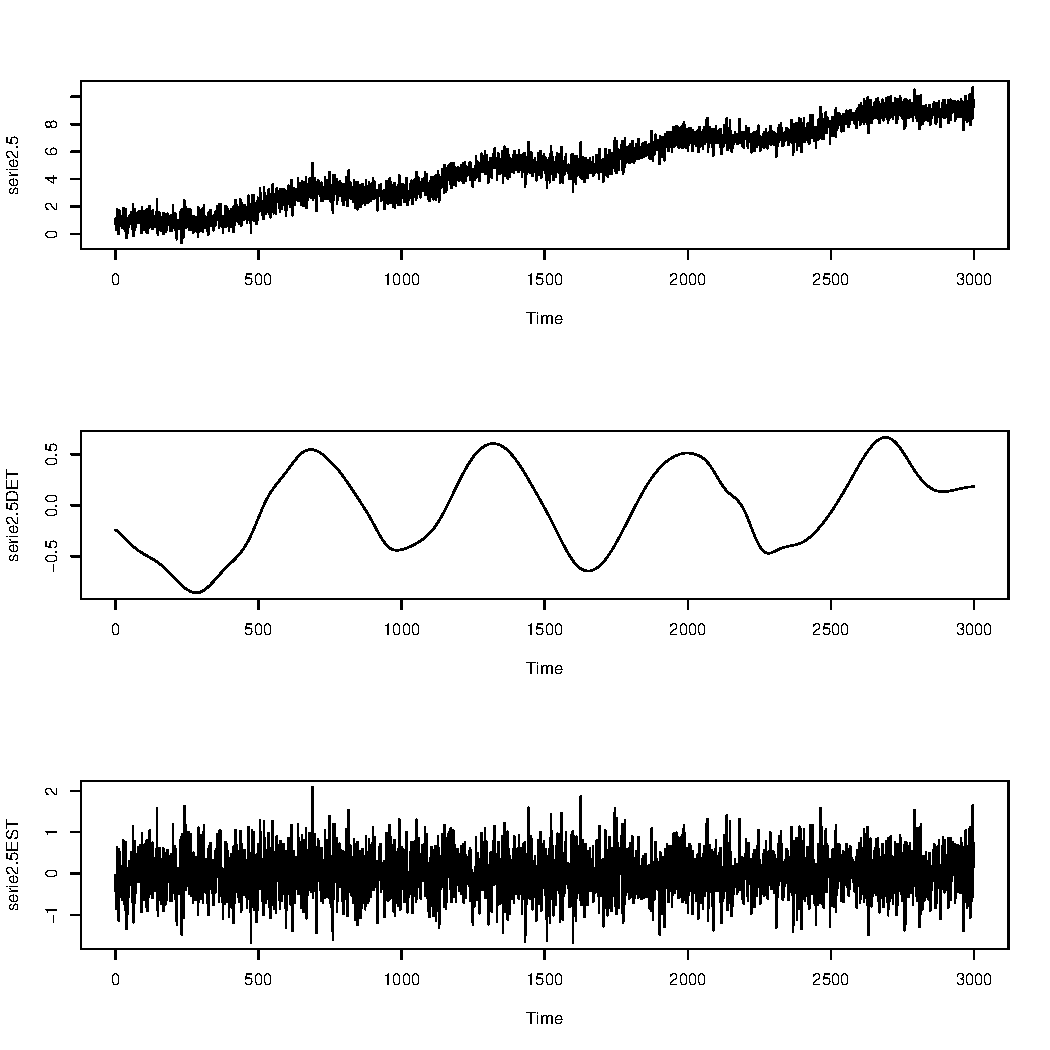
\includegraphics[scale=0.43]{serie2_5.pdf} \quad
  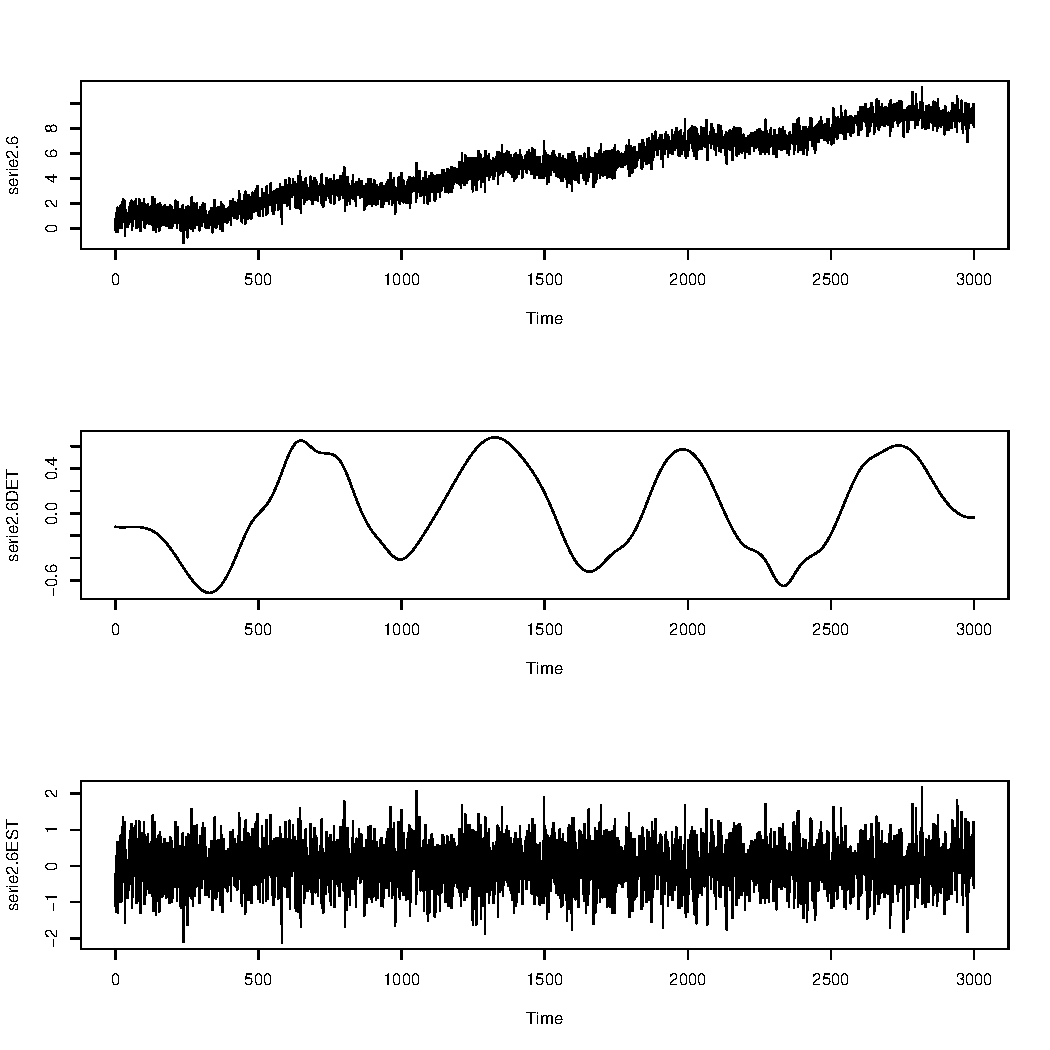
\includegraphics[scale=0.43]{serie2_6.pdf}
  \caption{Série 2.5 e Série 2.6}

\end{center}
\end{figure}

\graphicspath{{imagens/}}
\begin{figure}[H]
\begin{center}
  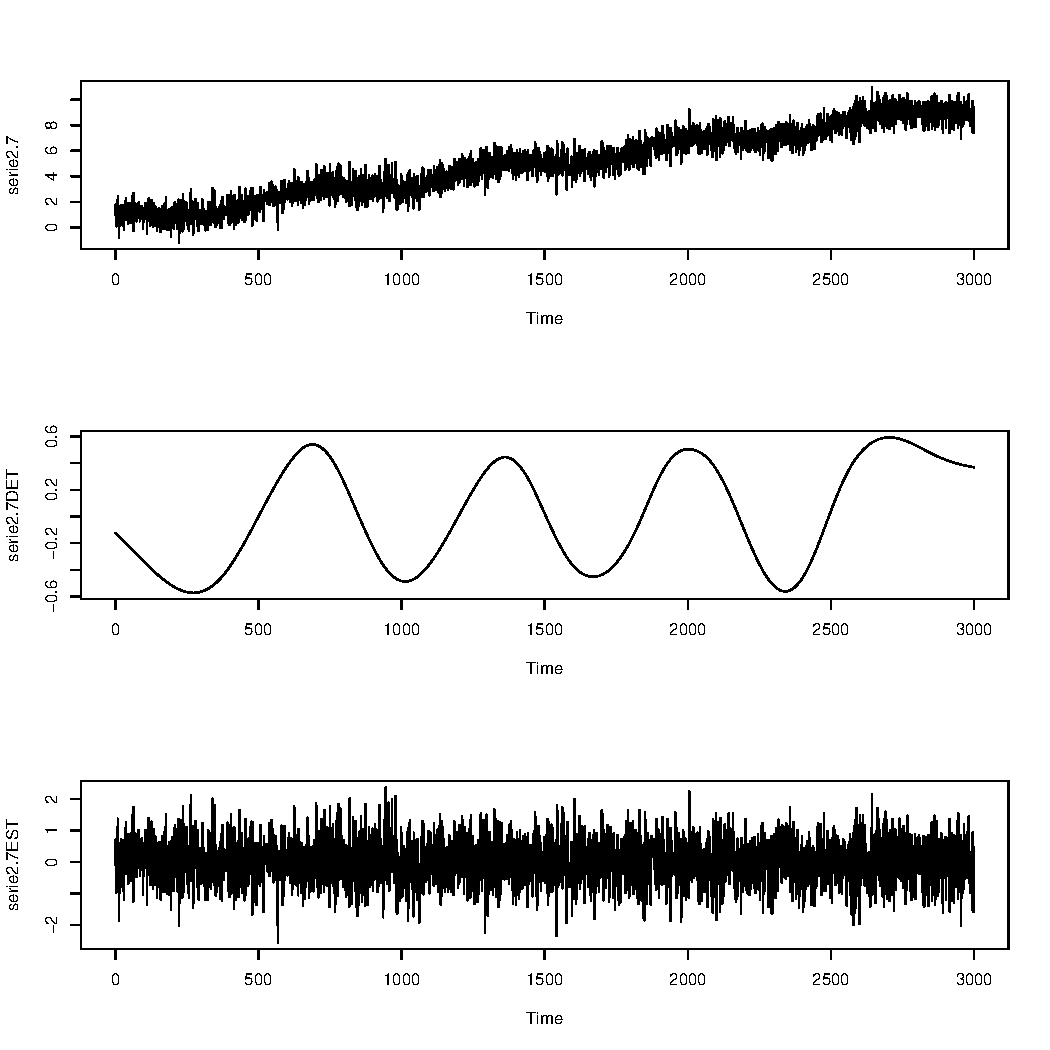
\includegraphics[scale=0.43]{serie2_7.pdf} \quad
  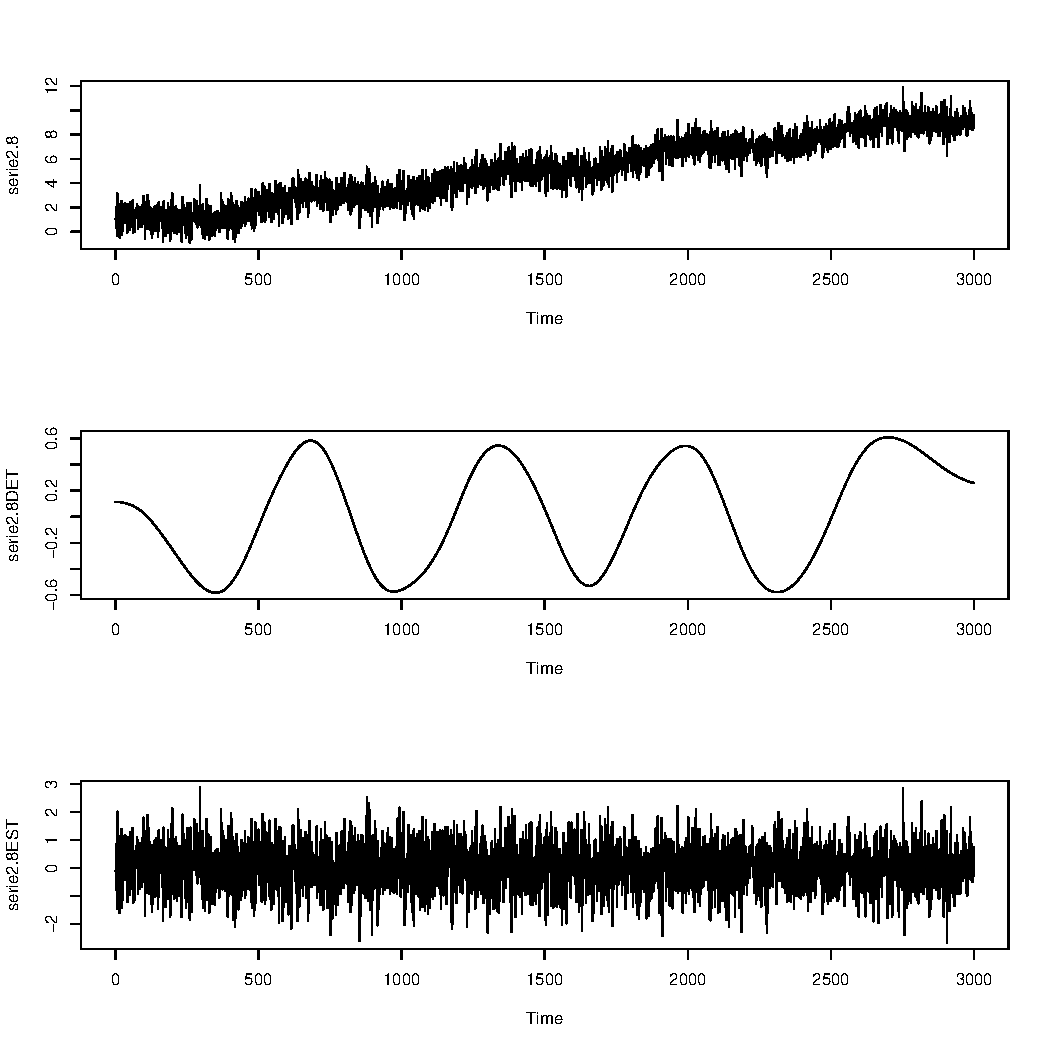
\includegraphics[scale=0.43]{serie2_8.pdf}
  \caption{Série 2.7 e Série 2.8}

\end{center}
\end{figure}

\graphicspath{{imagens/}}
\begin{figure}[H]
\begin{center}
  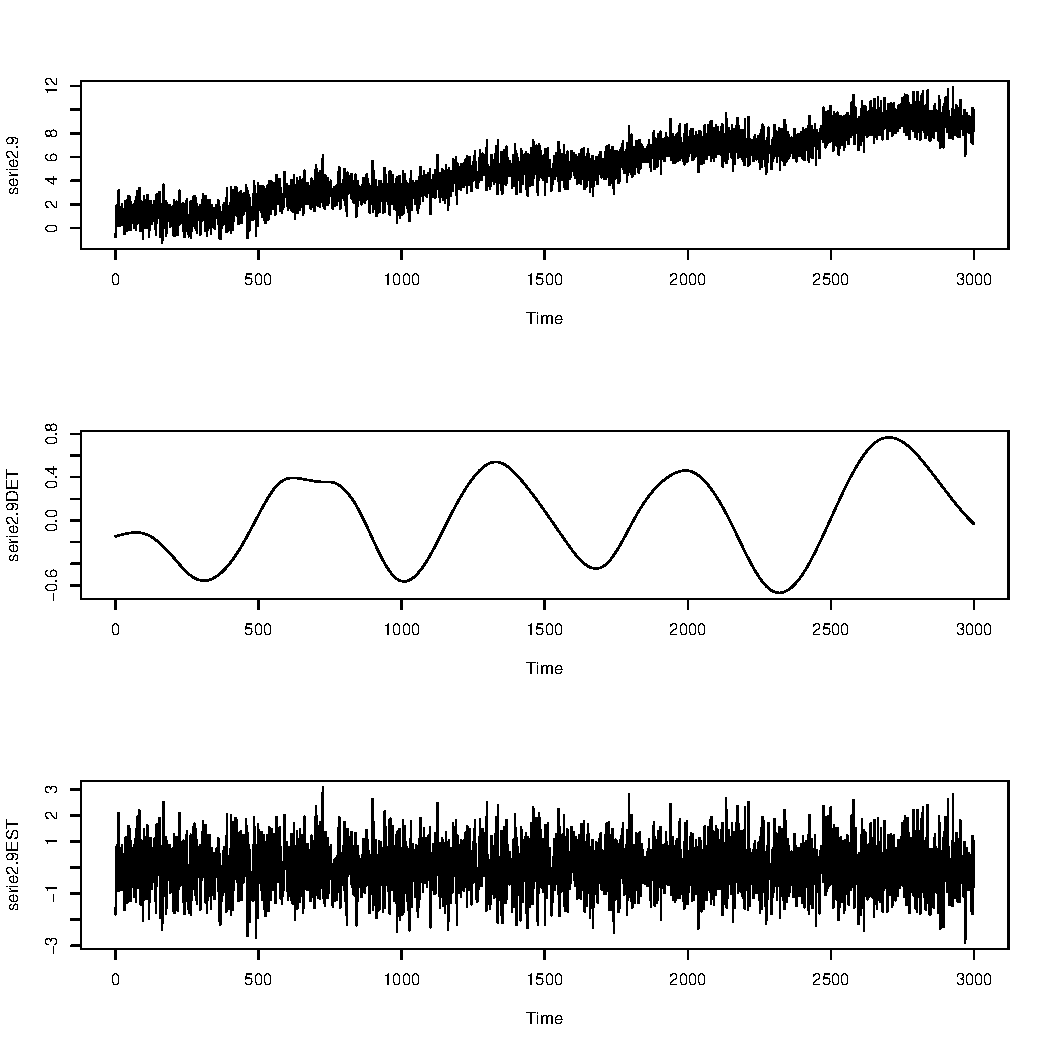
\includegraphics[scale=0.43]{serie2_9.pdf} \quad
  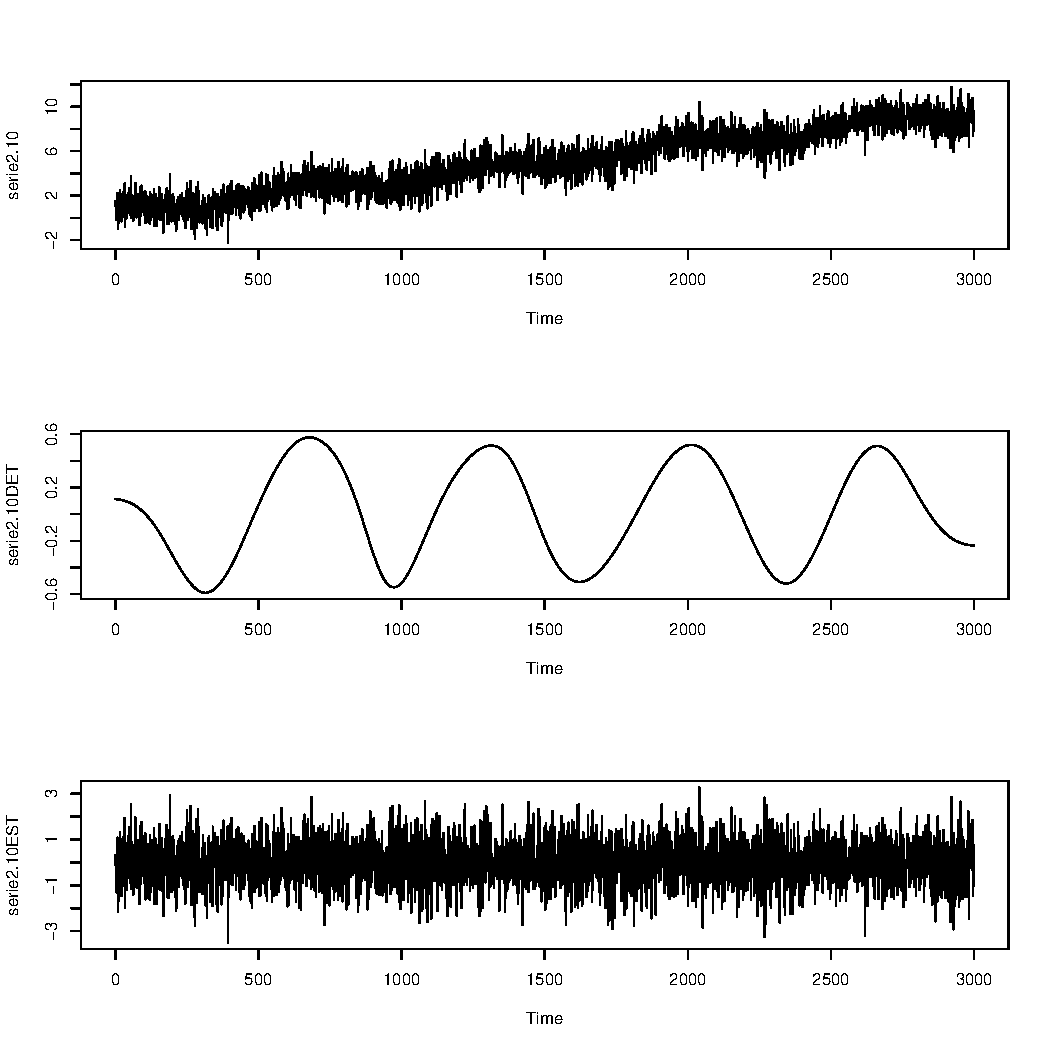
\includegraphics[scale=0.43]{serie2_10.pdf}
  \caption{Série 2.9 e Série 2.10}

\end{center}
\end{figure}

\section{Séries TIPO 3}
10 séries senoide com ruído ao longo da série.
\graphicspath{{imagens/}}
\begin{figure}[H]
\begin{center}
  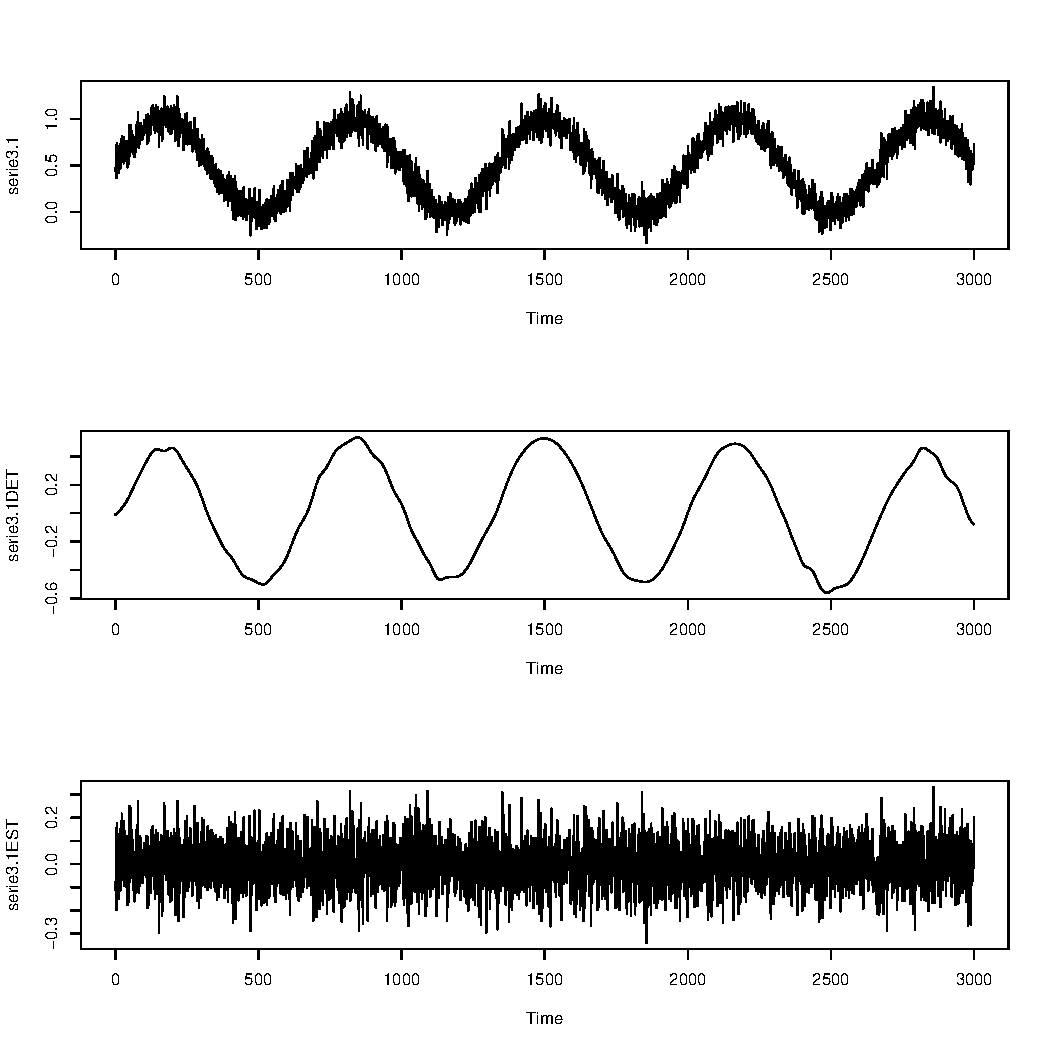
\includegraphics[scale=0.43]{serie3_1.pdf} \quad
  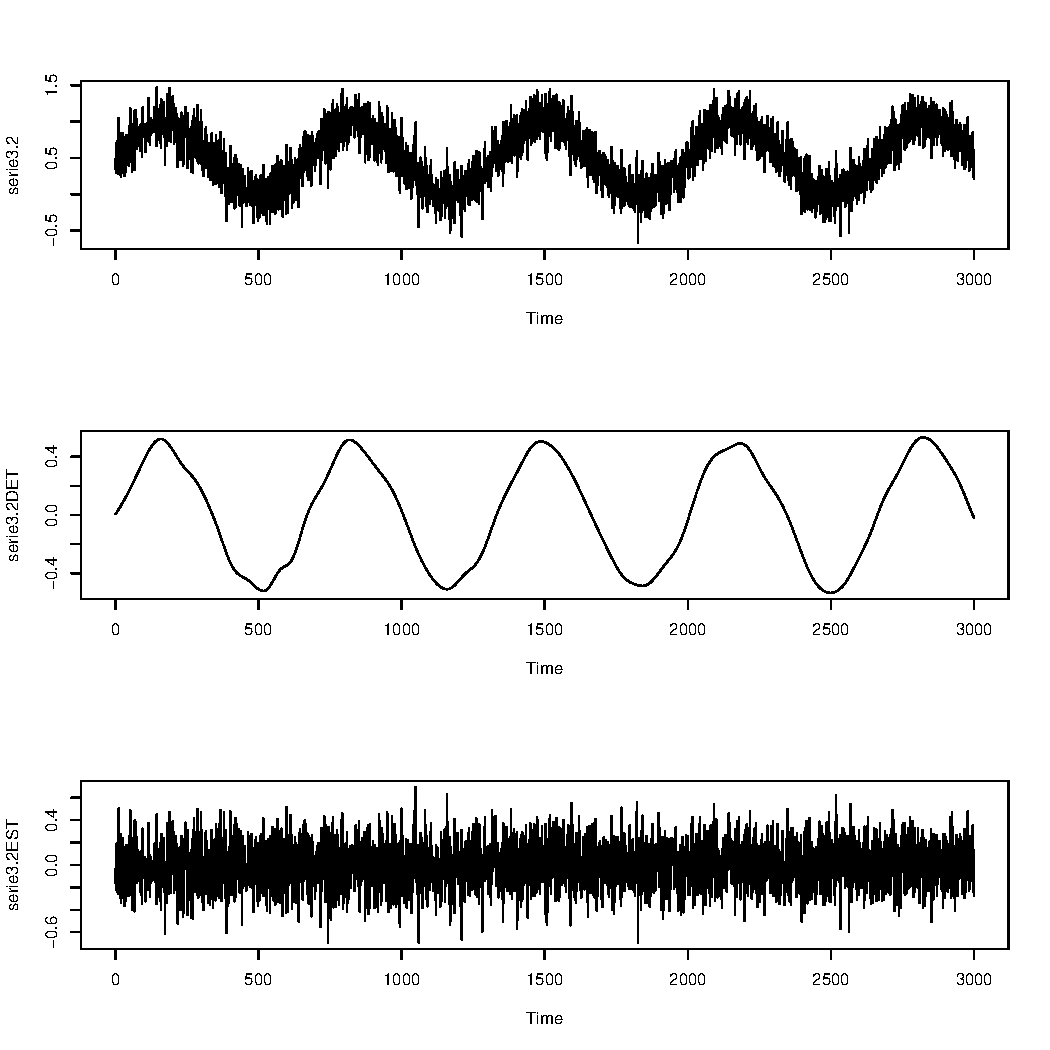
\includegraphics[scale=0.43]{serie3_2.pdf}
  \caption{Série 3.1 e Série 3.2}

\end{center}
\end{figure}

\graphicspath{{imagens/}}
\begin{figure}[H]
\begin{center}
  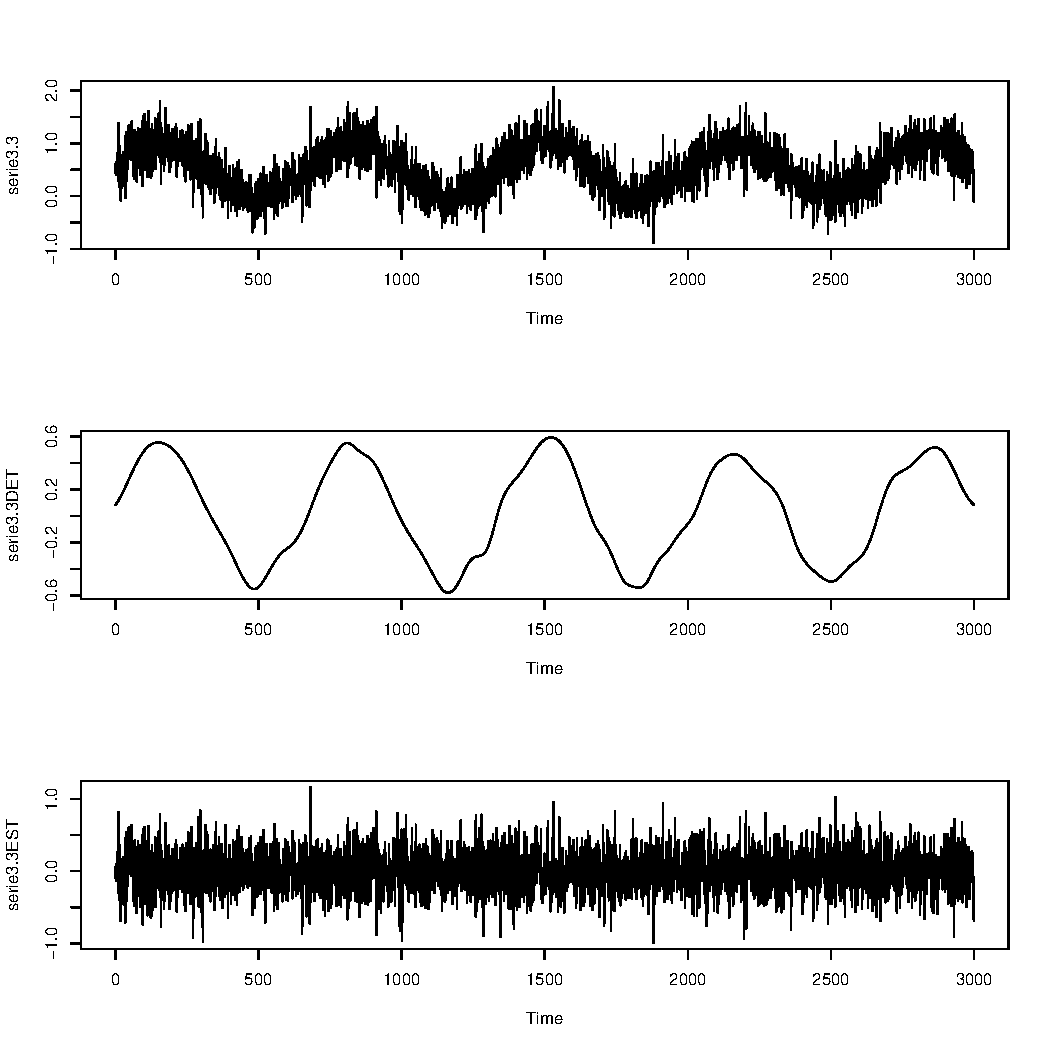
\includegraphics[scale=0.43]{serie3_3.pdf} \quad
  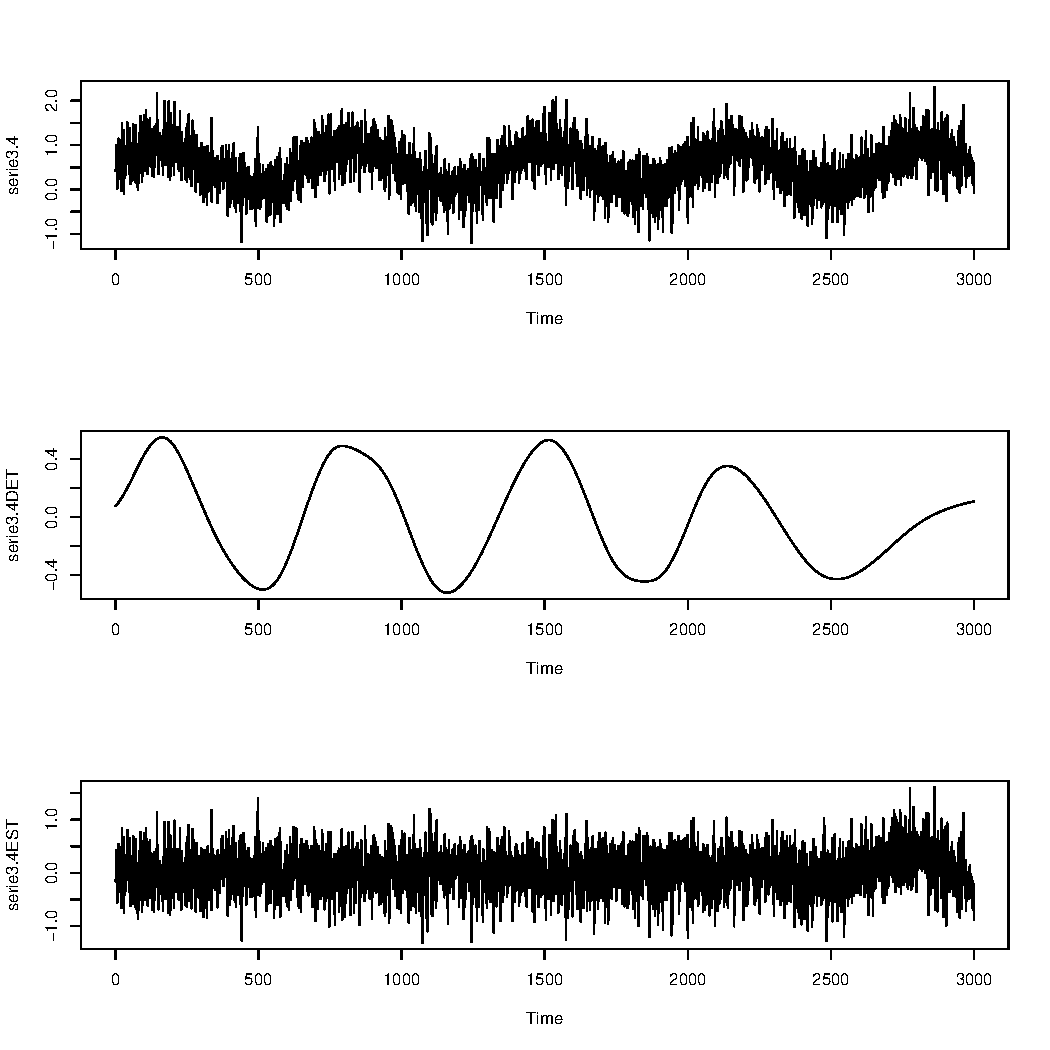
\includegraphics[scale=0.43]{serie3_4.pdf}
  \caption{Série 3.3 e Série 3.4}

\end{center}
\end{figure}

\graphicspath{{imagens/}}
\begin{figure}[H]
\begin{center}
  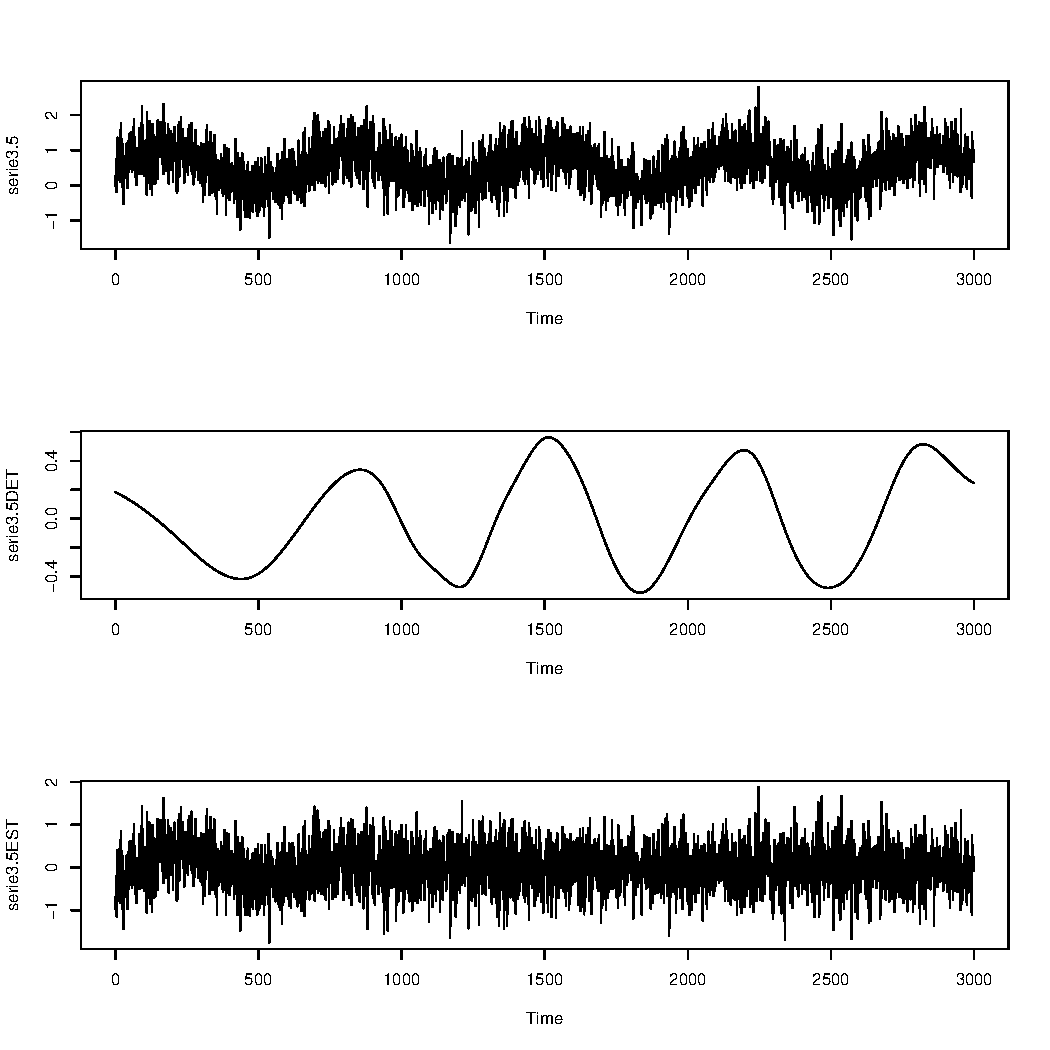
\includegraphics[scale=0.43]{serie3_5.pdf} \quad
  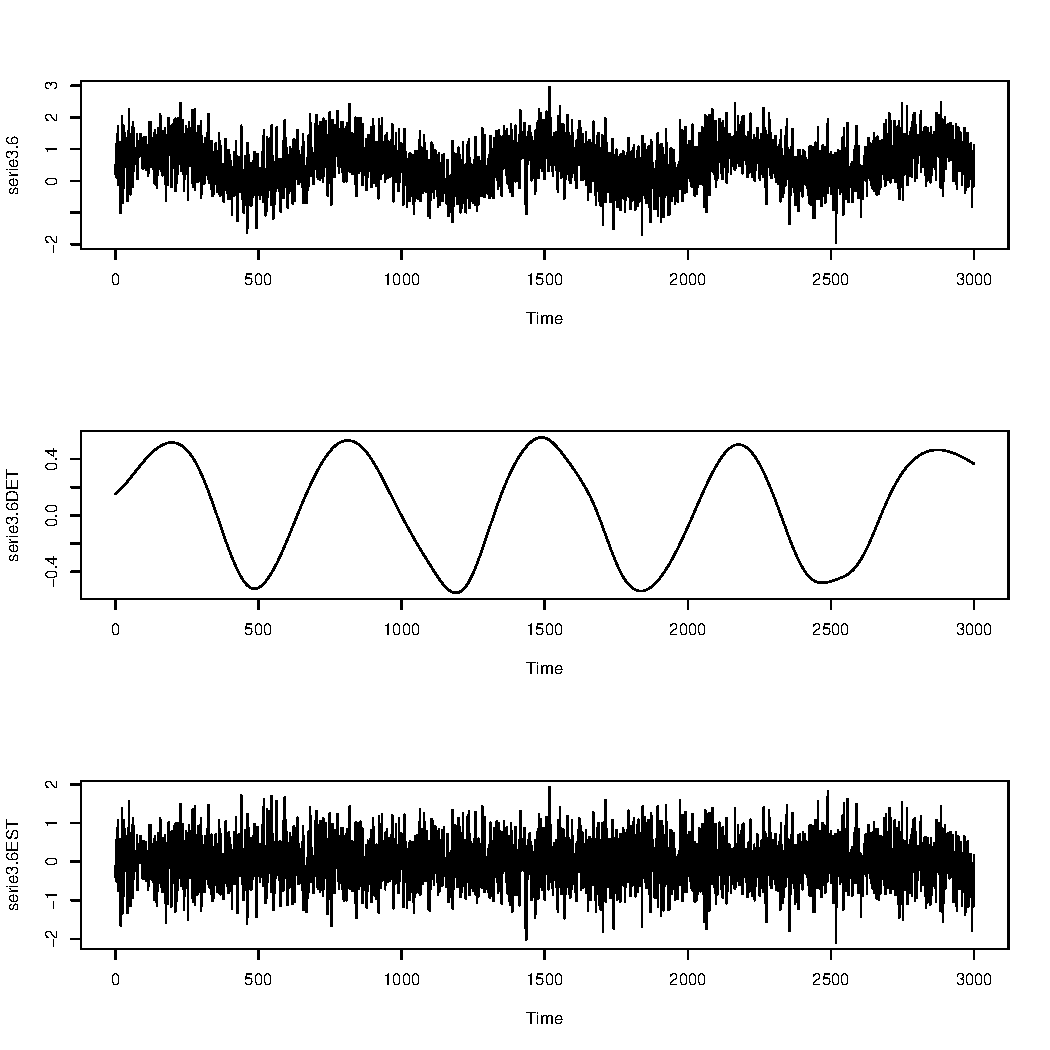
\includegraphics[scale=0.43]{serie3_6.pdf}
  \caption{Série 3.5 e Série 3.6}

\end{center}
\end{figure}

\graphicspath{{imagens/}}
\begin{figure}[H]
\begin{center}
  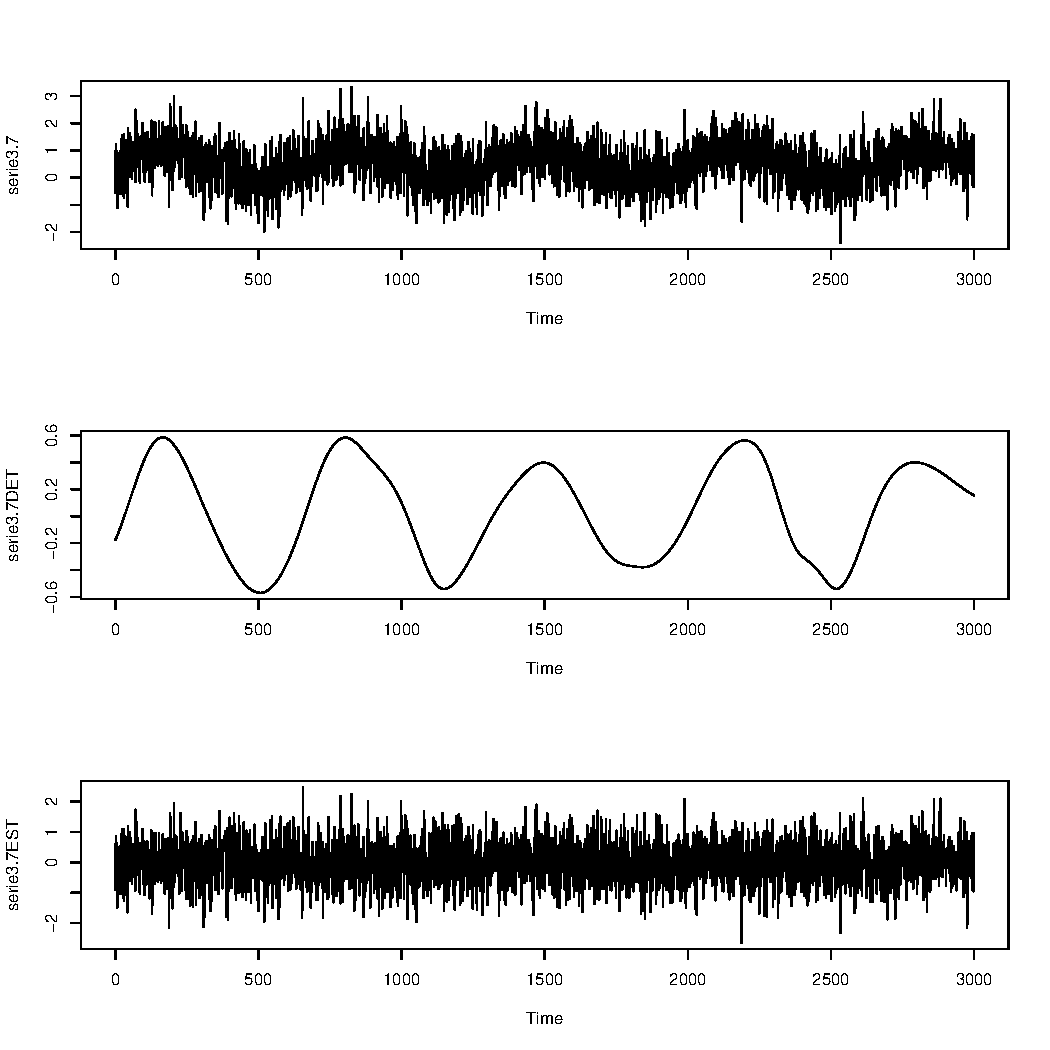
\includegraphics[scale=0.43]{serie3_7.pdf} \quad
  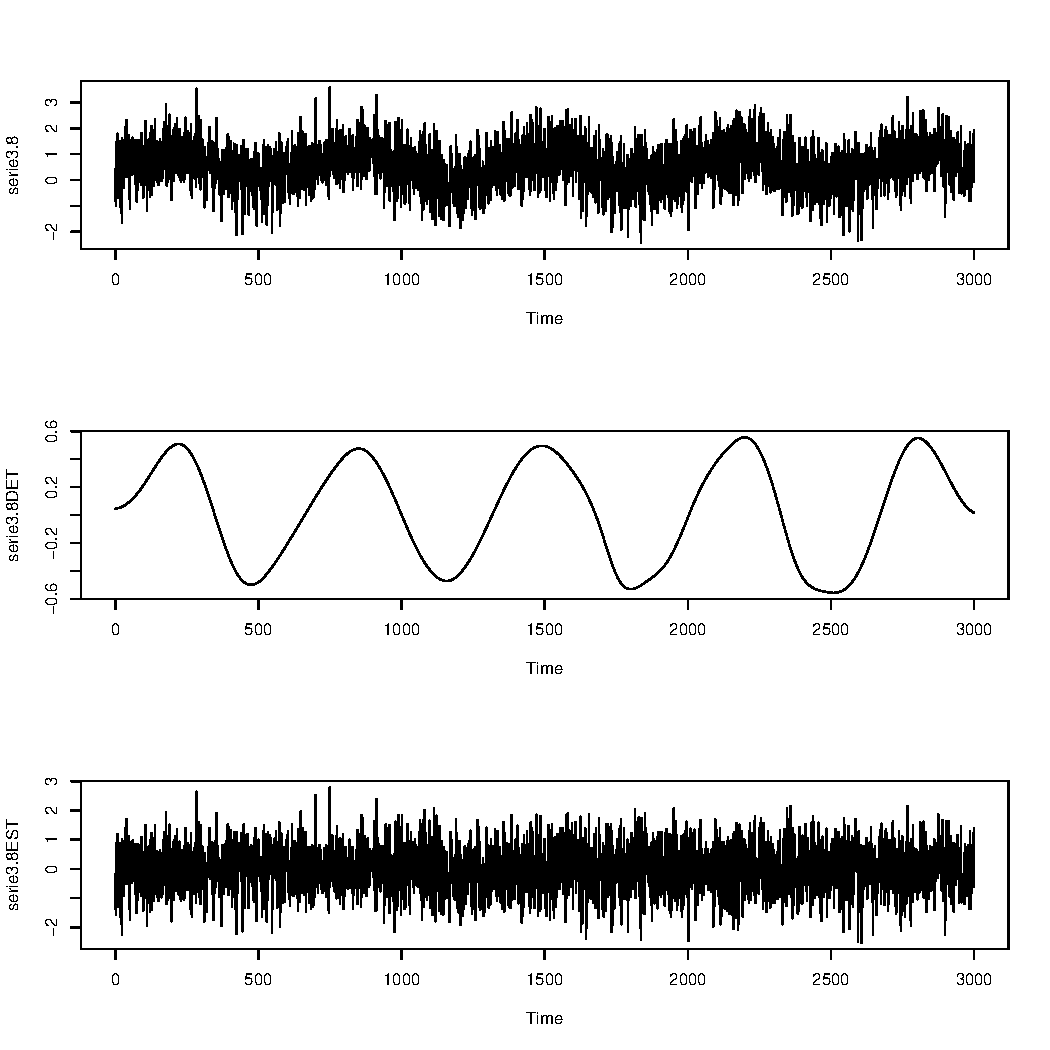
\includegraphics[scale=0.43]{serie3_8.pdf}
  \caption{Série 3.7 e Série 3.8}

\end{center}
\end{figure}

\graphicspath{{imagens/}}
\begin{figure}[H]
\begin{center}
  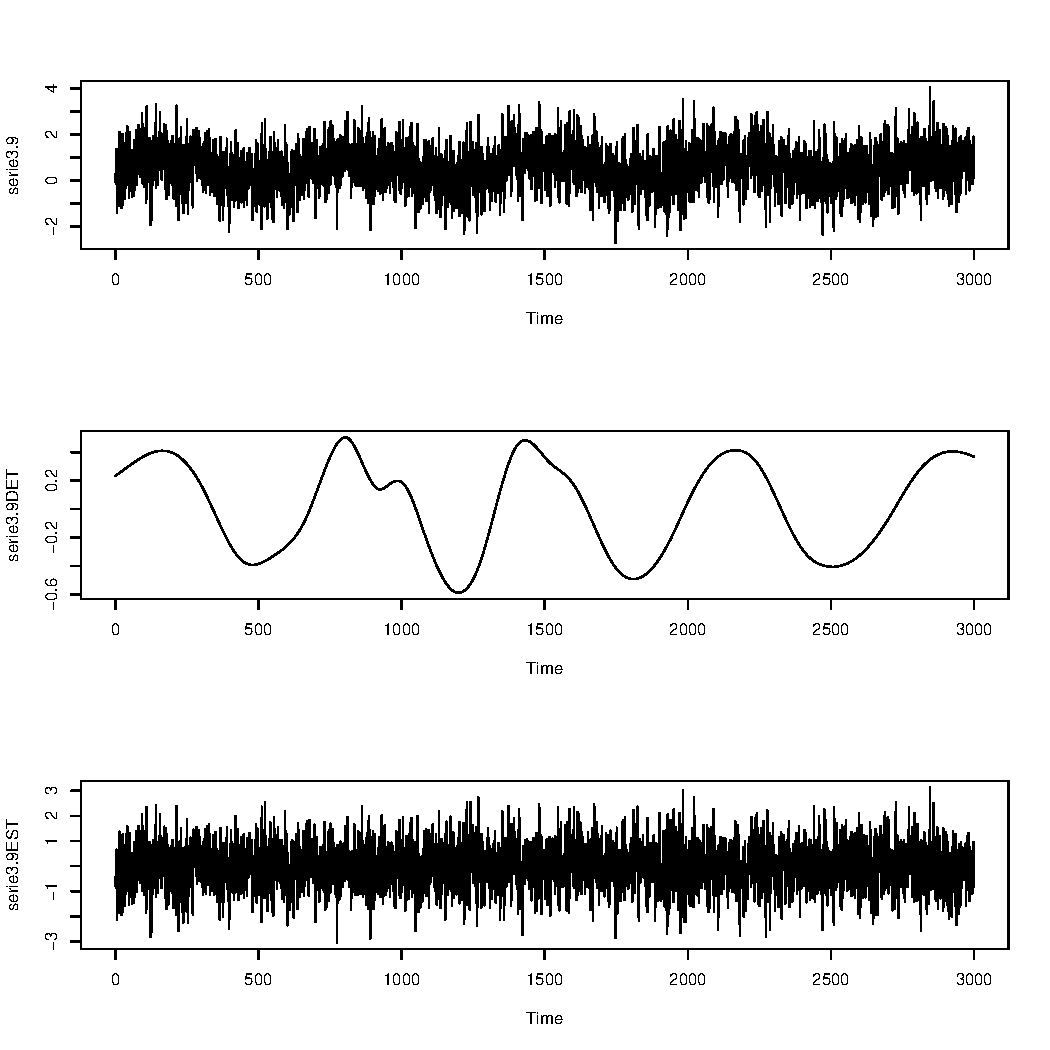
\includegraphics[scale=0.43]{serie3_9.pdf} \quad
  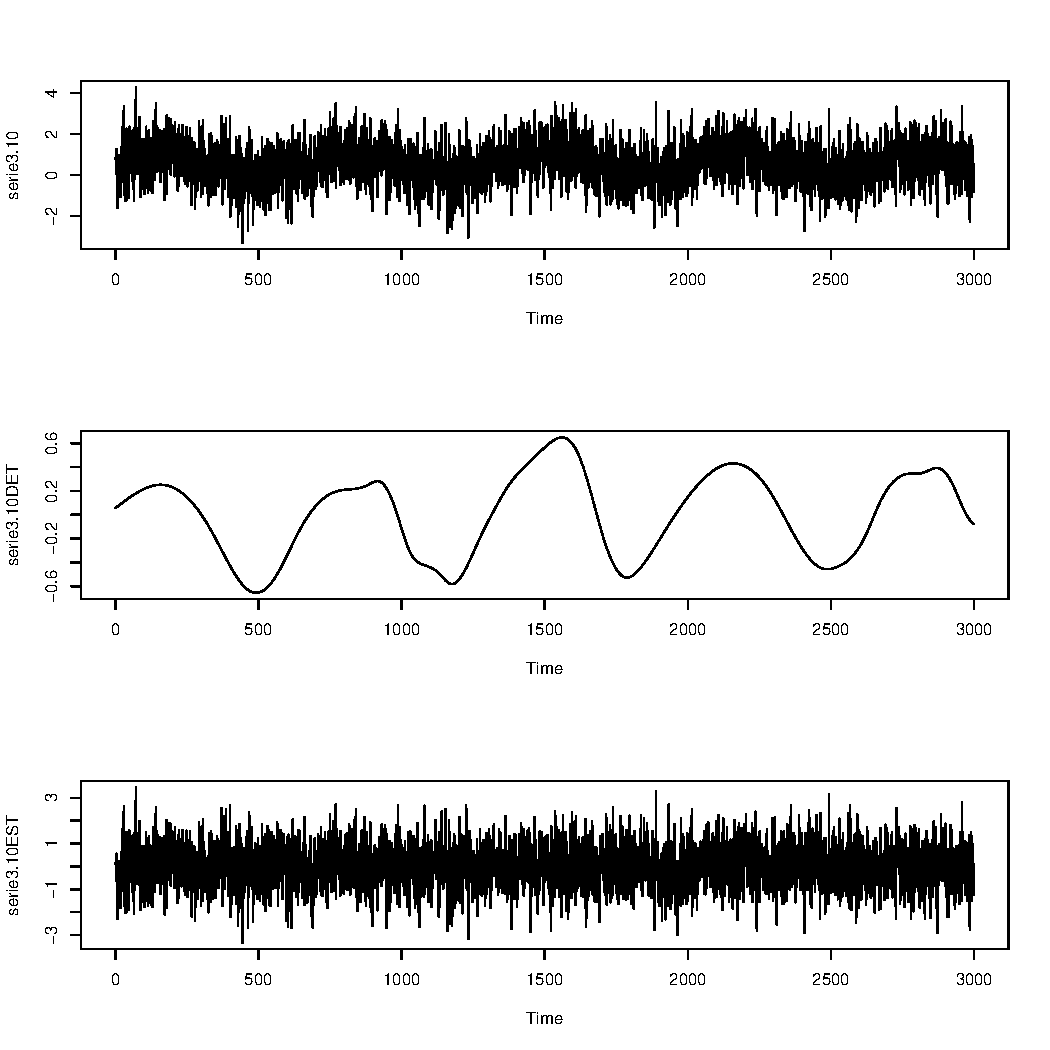
\includegraphics[scale=0.43]{serie3_10.pdf}
  \caption{Série 3.9 e Série 3.10}

\end{center}
\end{figure}

\section{Séries TIPO 4}
10 séries senoide com ruído ao longo da série e tendência.
\graphicspath{{imagens/}}
\begin{figure}[H]
\begin{center}
  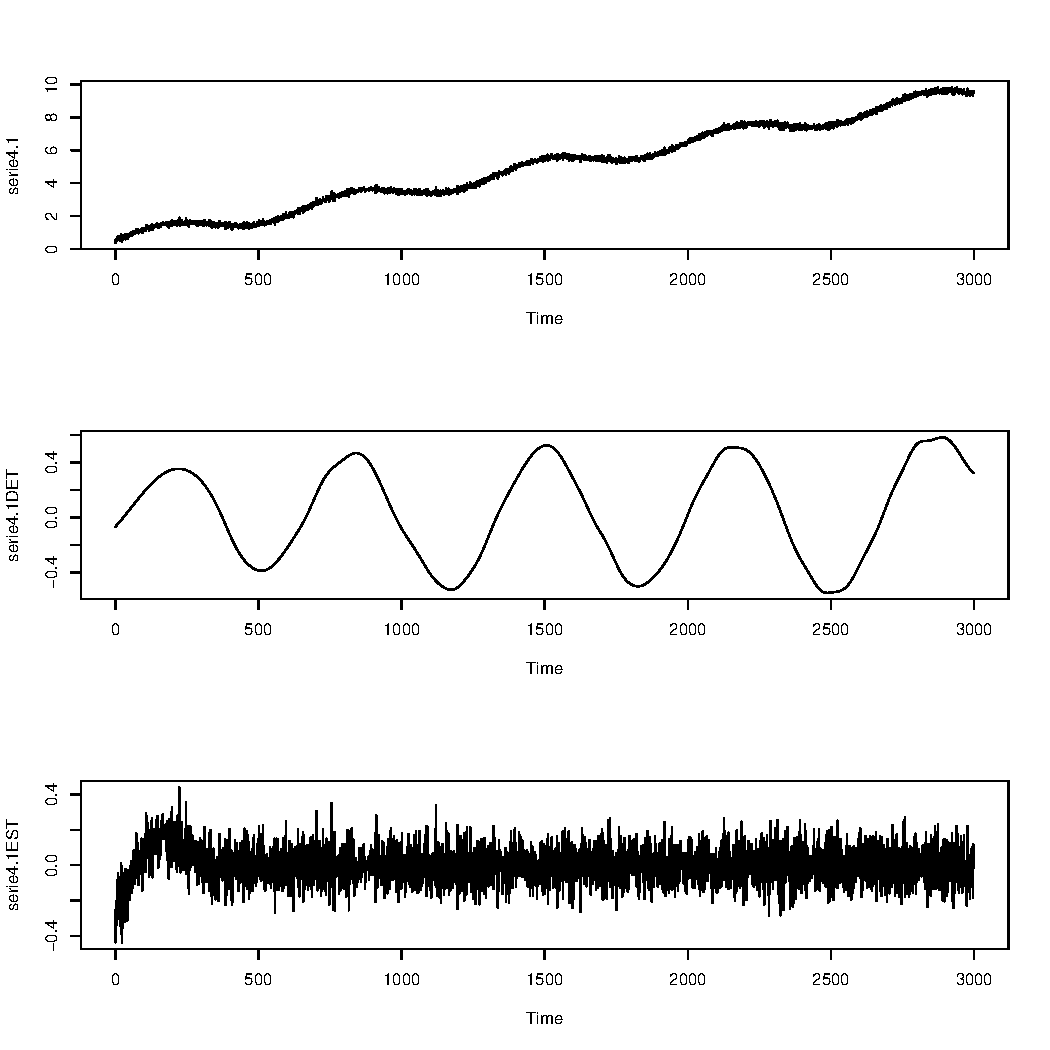
\includegraphics[scale=0.43]{serie4_1.pdf} \quad
  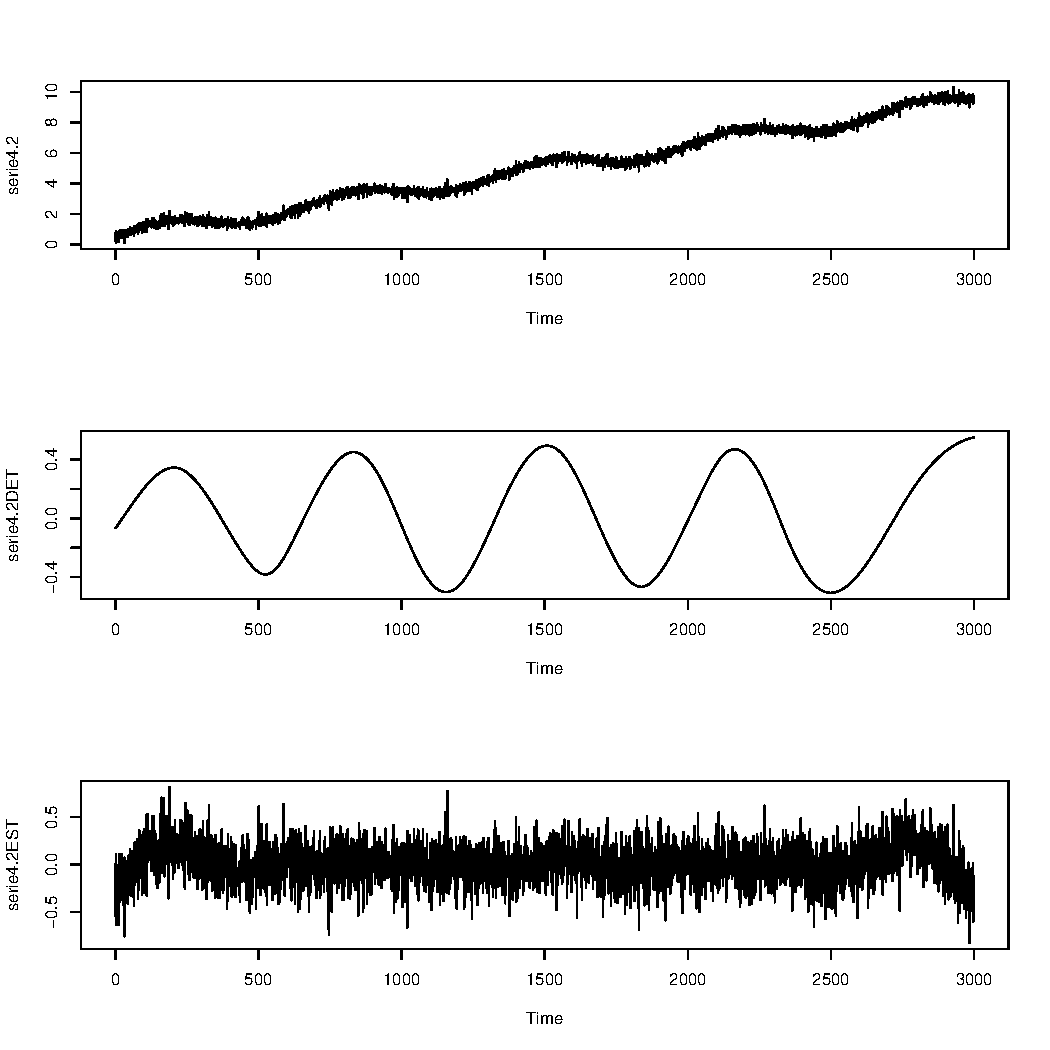
\includegraphics[scale=0.43]{serie4_2.pdf}
  \caption{Série 4.1 e Série 4.2}
\end{center}
\end{figure}

\graphicspath{{imagens/}}
\begin{figure}[H]
\begin{center}
  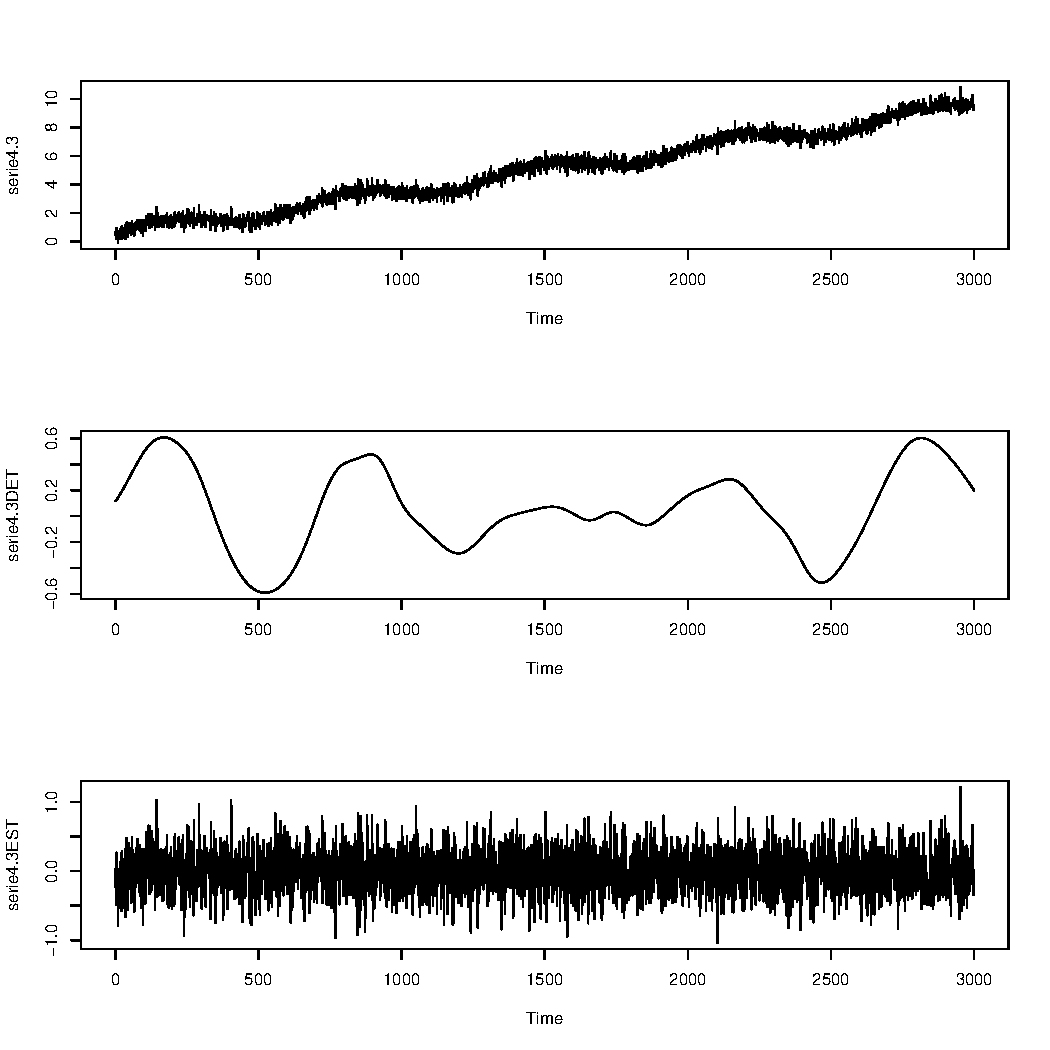
\includegraphics[scale=0.43]{serie4_3.pdf} \quad
 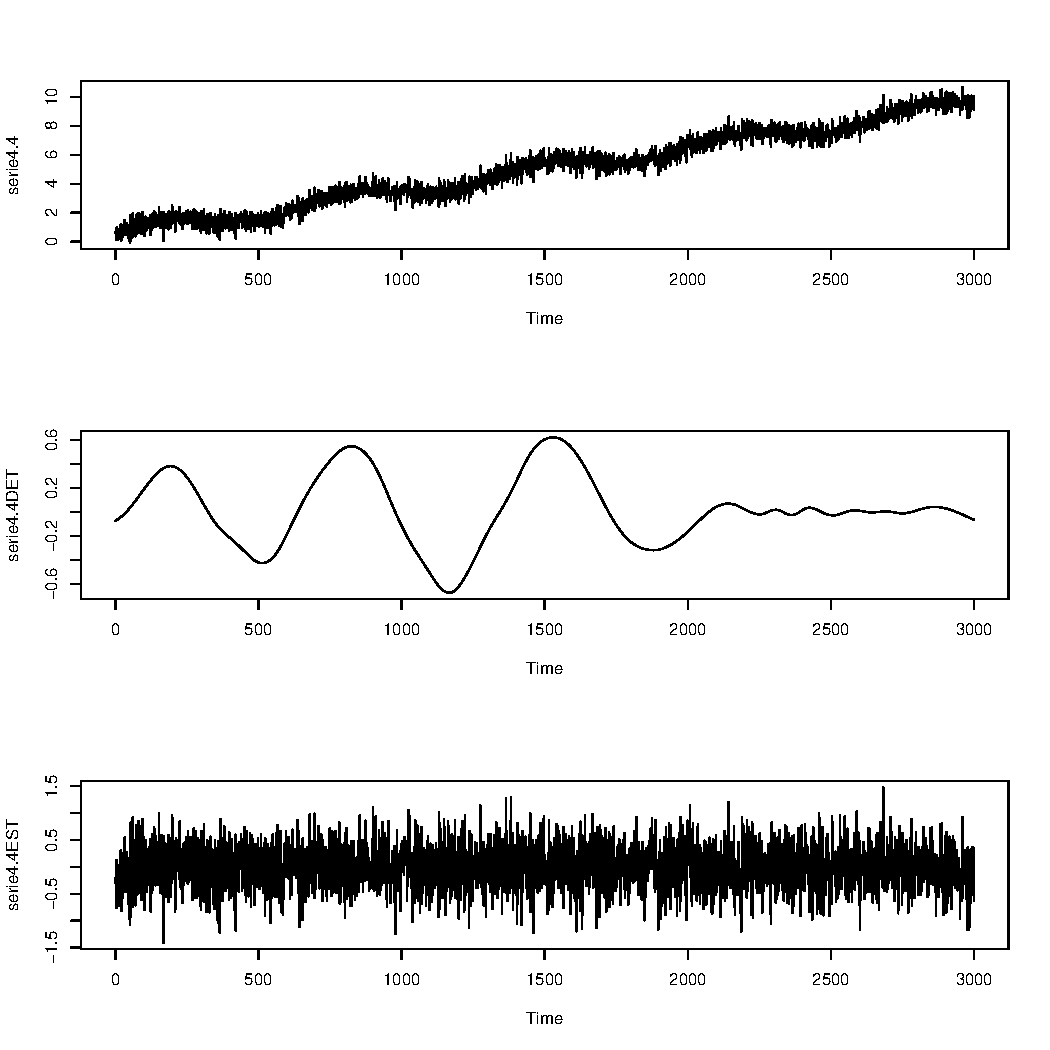
\includegraphics[scale=0.43]{serie4_4.pdf}
 \caption{Série 4.3 e Série 4.4}

\end{center}
\end{figure}

\graphicspath{{imagens/}}
\begin{figure}[H]
\begin{center}
  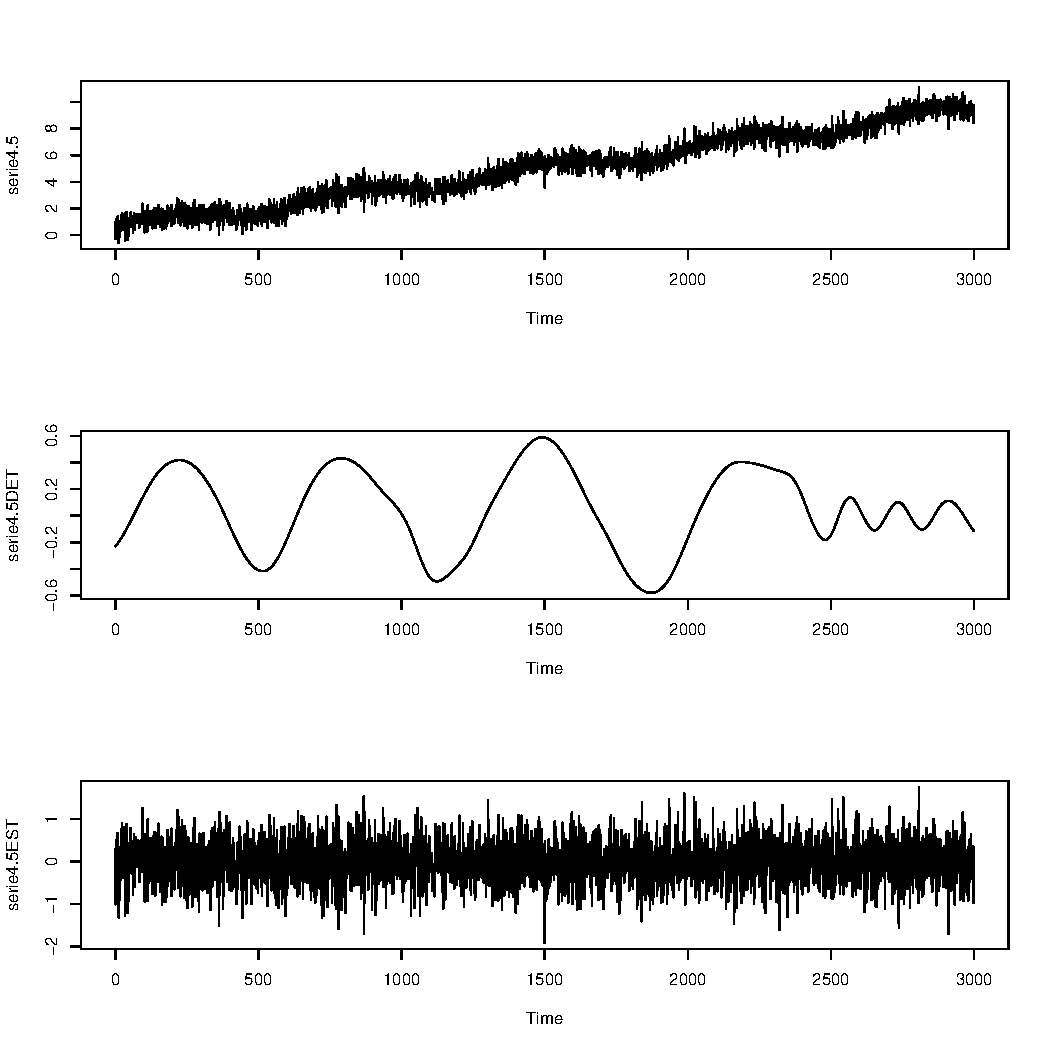
\includegraphics[scale=0.43]{serie4_5.pdf} \quad
  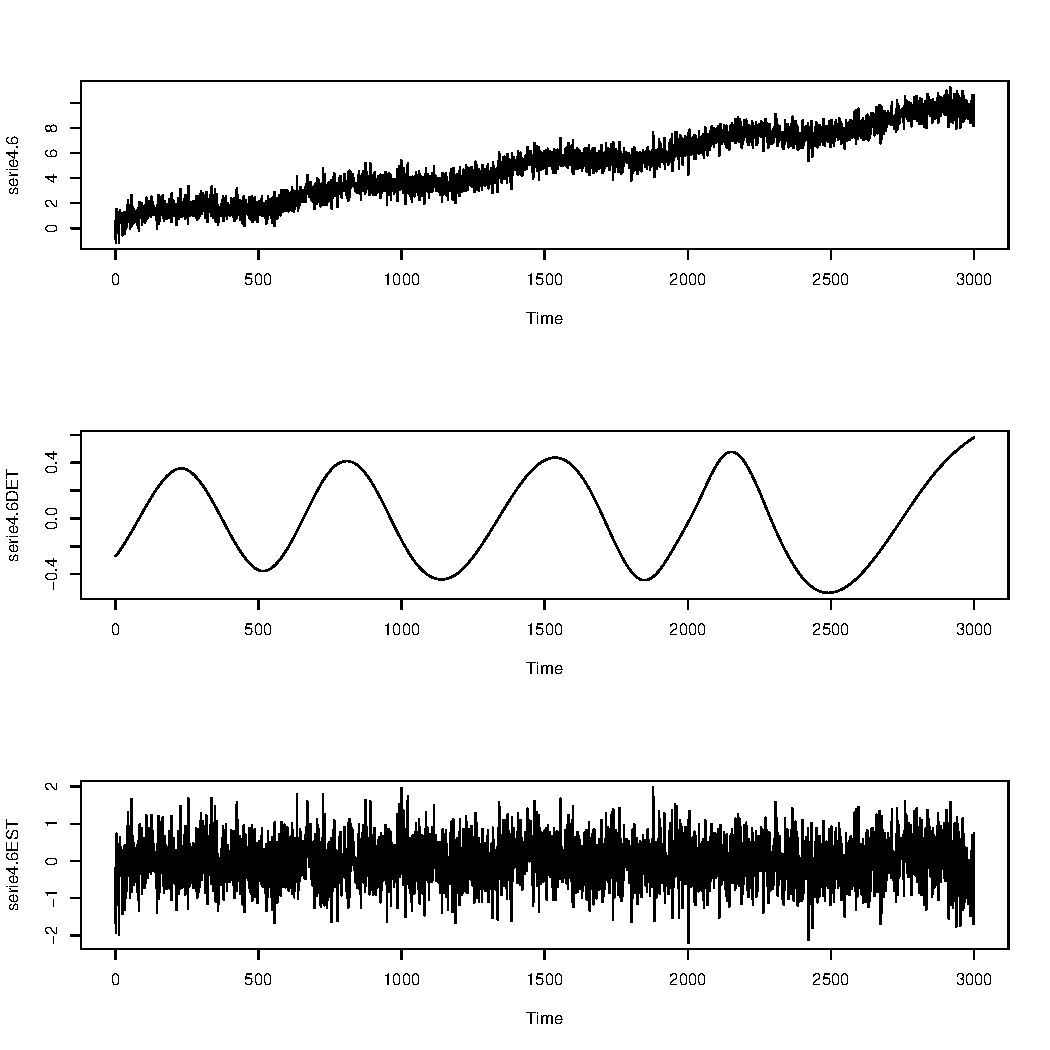
\includegraphics[scale=0.43]{serie4_6.pdf}
 \caption{Série 4.5 e Série 4.6}

\end{center}
\end{figure}

\graphicspath{{imagens/}}
\begin{figure}[H]
\begin{center}
  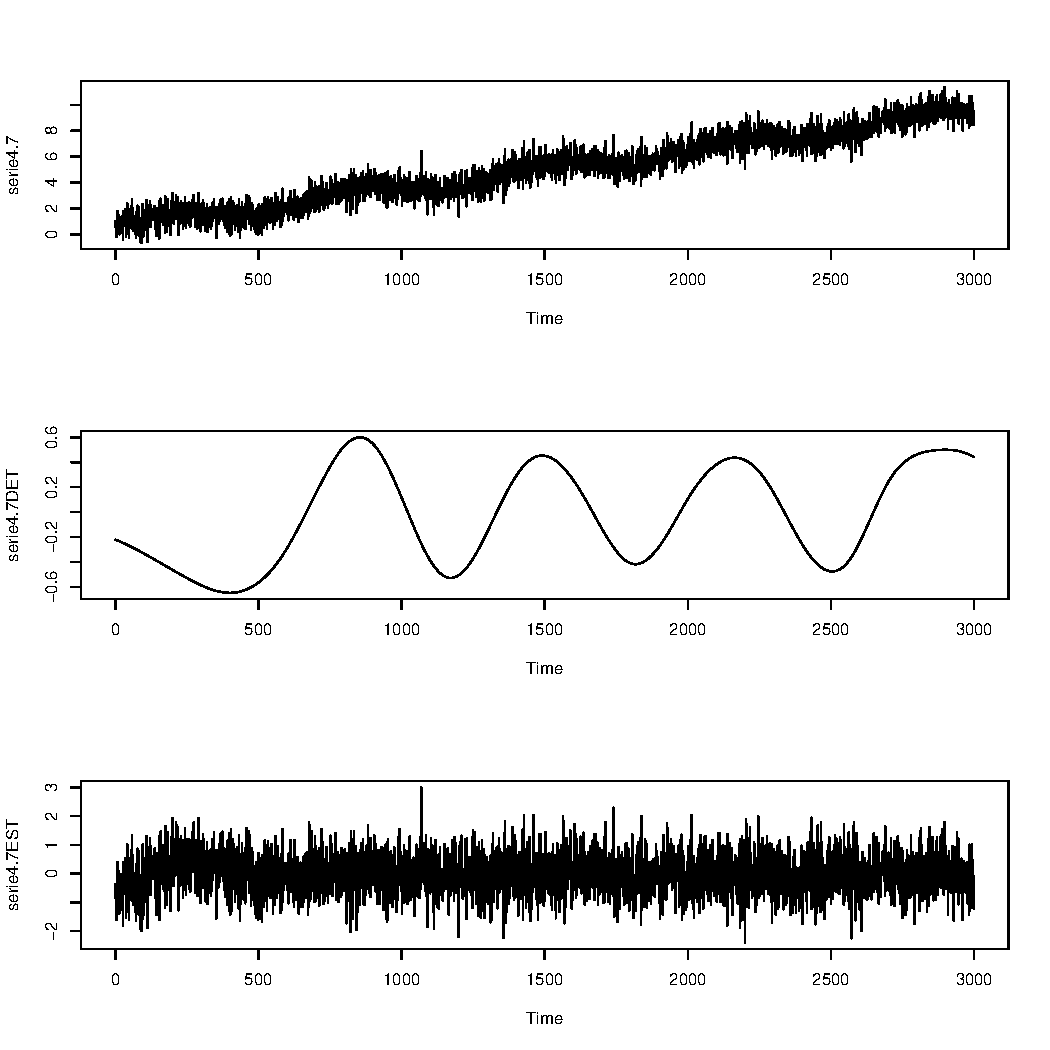
\includegraphics[scale=0.43]{serie4_7.pdf} \quad
  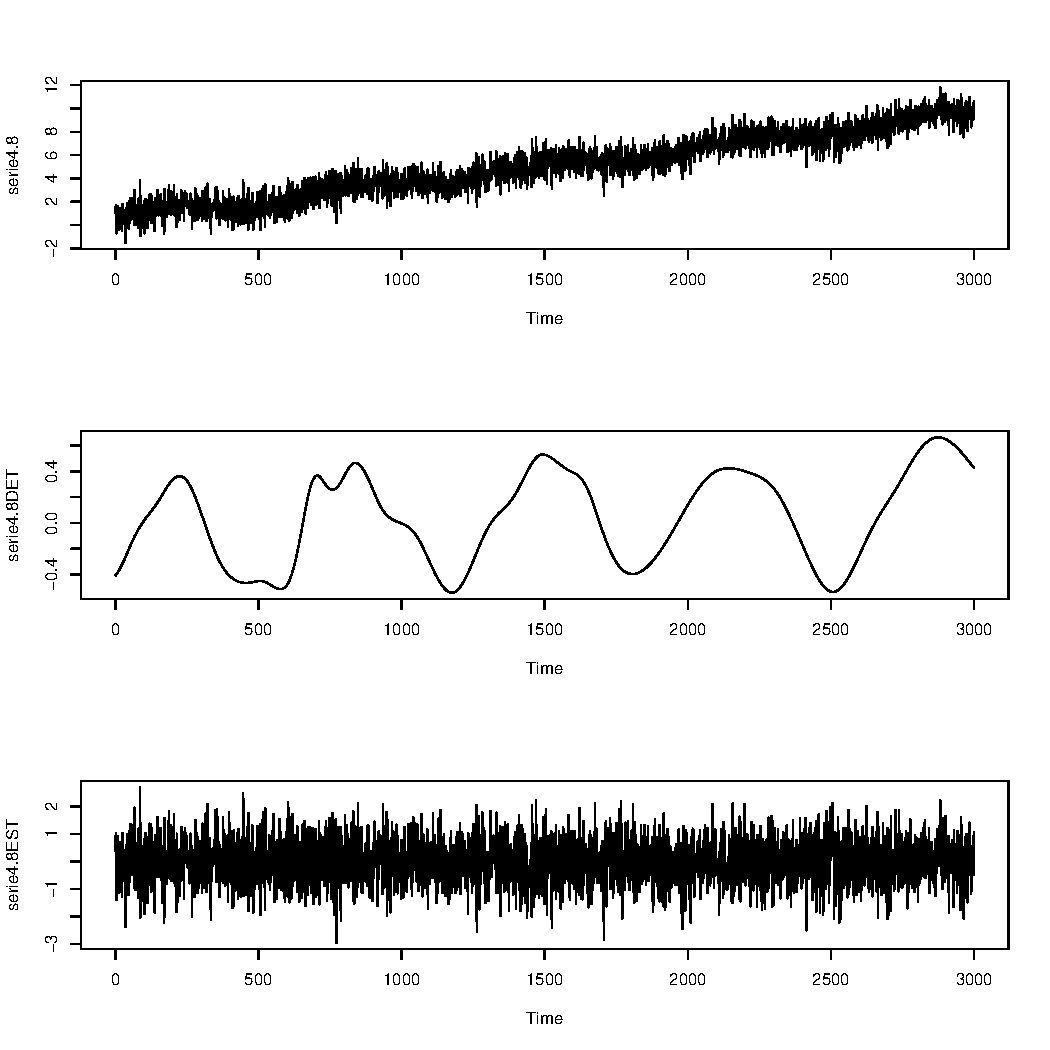
\includegraphics[scale=0.43]{serie4_8.pdf}
  \caption{Série 4.7 e Série 4.8}

\end{center}
\end{figure}

\graphicspath{{imagens/}}
\begin{figure}[H]
\begin{center}
  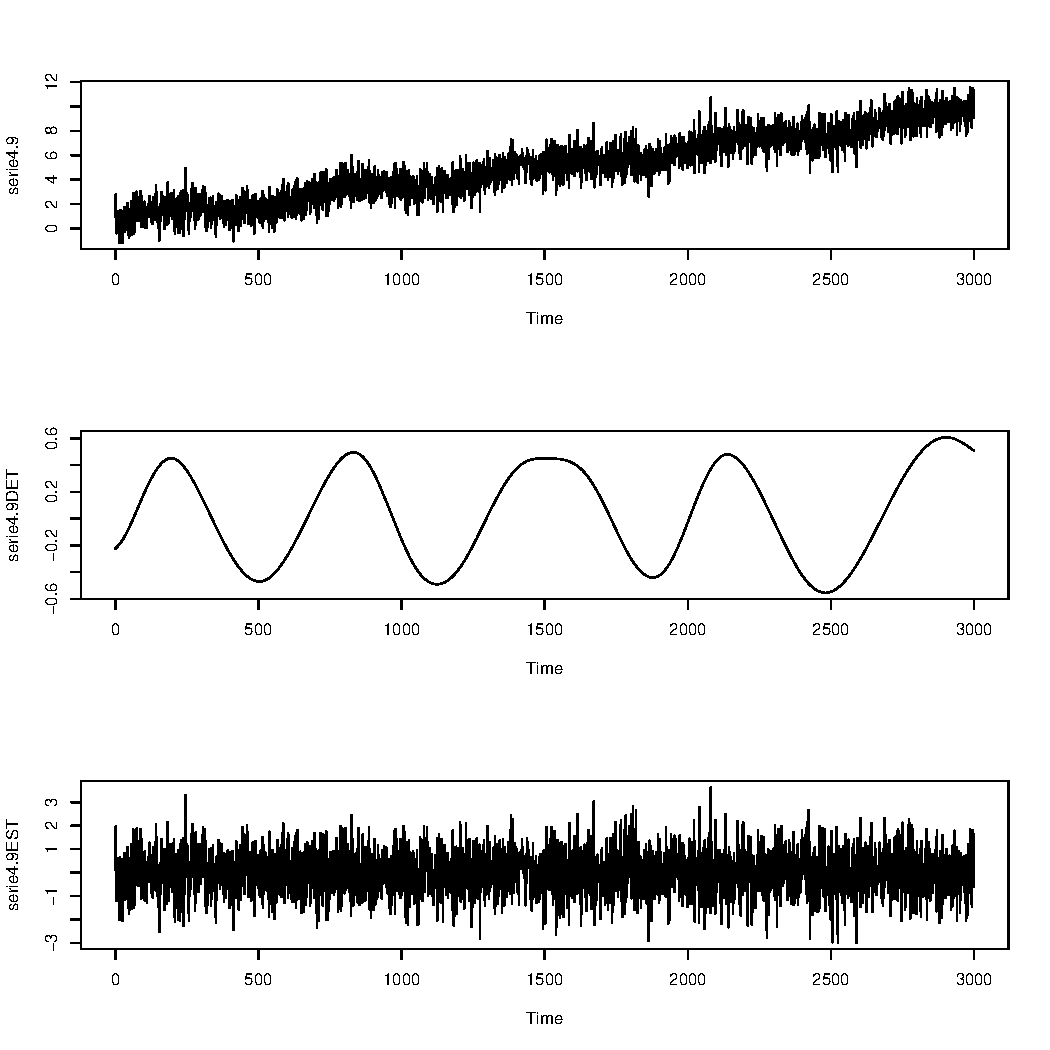
\includegraphics[scale=0.43]{serie4_9.pdf} \quad
  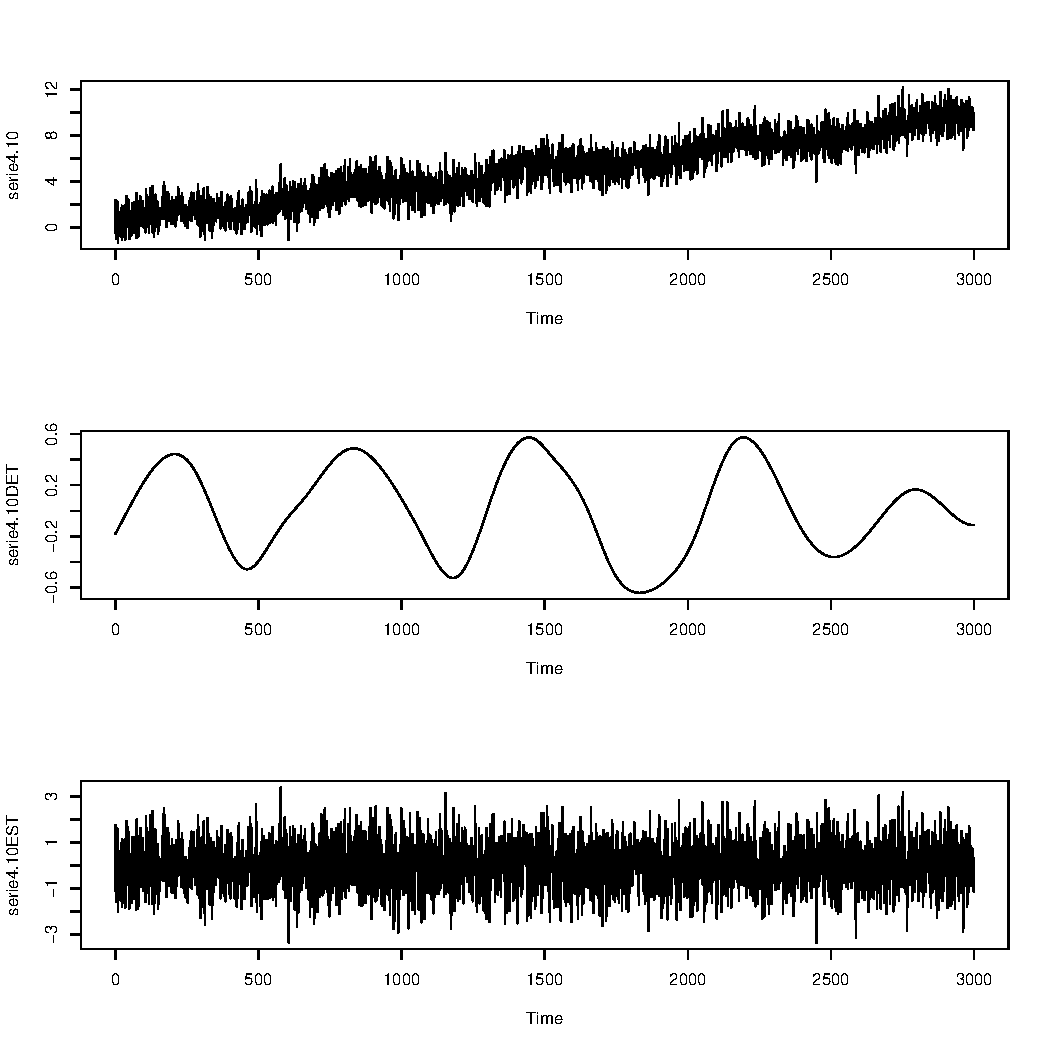
\includegraphics[scale=0.43]{serie4_10.pdf}
  \caption{Série 4.9 e Série 4.10}
\end{center}
\end{figure}
\section{Considerações Finais}
Foram apresentadas as séries temporais utilizadas neste trabalho experimental e suas respactivas decomposições.
% \include{apendice2}
% ...
% \include{apendiceM}

%% Fim do documento
\end{document}
%------------------------------------------------------------------------------------------%
